% ============================================================
%  Semana 7 · Clase 13: Power BI, carga, transformación y modelo de datos
%  Curso: Análisis y Visualización de Datos para la Toma de Decisiones
%
%  Formato de la sesión (3 h), en forma de guía paso a paso:
%    Hora 1. De Python a Power BI Desktop: interfaz y carga de datos
%    Hora 2. Power Query: limpiar y transformar la hoja Socios
%    Hora 3. Modelo estrella: hechos, dimensiones, relaciones y DAX
%
%  Datos: datos/gimnasio_vitalis.xlsx (generado con
%  ../../../scripts/semana07-clase13_datos.py)
%
%  Las capturas de figuras/ms-learn/ provienen de Microsoft Learn y se
%  usan sin modificar, según la política de Microsoft para capturas de
%  pantalla de sus productos ("Used with permission from Microsoft").
%
%  Compilar (dos veces) directamente desde esta carpeta:
%    xelatex semana07-clase13.tex
%    xelatex semana07-clase13.tex
% ============================================================
\documentclass[aspectratio=169,11pt]{beamer}

\usepackage{../../../plantilla/beamerthemeesumer}
\usetheme{esumer}

\usepackage[spanish,es-noshorthands]{babel}
\usepackage{booktabs}
\usepackage{graphicx}
\usepackage{array}
\newcolumntype{L}[1]{>{\raggedright\arraybackslash}p{#1}}
\usetikzlibrary{arrows.meta,shapes.multipart,positioning,calc}

% ---------------- DATOS DE LA CLASE ----------------
\title{Power BI: carga, transformación y modelo de datos}
\subtitle{Guía paso a paso con los datos del Gimnasio Vitalis}
\author{Docente: Cristian A. Jimenez C., MSc}
\date{Oct 20 al 25}

\setmodulo{Módulo 3: Experimentar (Visualización e Insights)}
\setsemana{7}
\setclase{13}
\setfechaclase{Oct 20 al 25}
\setmodalidad{Virtual}
% -----------------------------------------------------

\graphicspath{{figuras/}}

% Pie de cada captura: producto, página de origen y la frase que exige Microsoft
\newcommand{\fuente}[2]{%
  \par\vspace{1pt}{\fontsize{5.5}{6.5}\selectfont\color{black!55}%
  Captura de Microsoft Power BI Desktop. Guía oficial de este paso:
  \href{#2}{\color{esumerOrange}«#1»}. Used with permission from Microsoft.\par}}

% Número de paso
\newcommand{\npaso}[1]{\tikz[baseline=(n.base)]\node[circle,fill=esumerOrange,
  text=white,font=\bfseries\footnotesize,inner sep=0pt,minimum size=0.48cm](n){#1};}

% Fórmula (M o DAX) en un recuadro sin título
\newcommand{\codigo}[1]{\par\smallskip\noindent\colorbox{esumerGray!70}{\parbox{\dimexpr\linewidth-2\fboxsep\relax}{\scriptsize\ttfamily #1}}\par\smallskip}

% Menú de Power BI: nombre en español (nombre en inglés)
\newcommand{\menu}[2]{\textbf{#1} {\color{black!55}(#2)}}

\newcommand{\urlconsultas}{https://learn.microsoft.com/es-es/power-bi/transform-model/desktop-query-overview}
\newcommand{\urlconectar}{https://learn.microsoft.com/es-es/power-bi/connect-data/desktop-quickstart-connect-to-data}
\newcommand{\urlinstalar}{https://learn.microsoft.com/es-es/power-bi/fundamentals/desktop-get-the-desktop}
\newcommand{\urldatos}{https://github.com/craljimenez/An-lisis_y_Visualizacion_de_Datos_para_la_Toma_de_Decisiones/raw/main/clases/semana07-clase13-powerbi-carga-transformacion-modelo/datos/gimnasio_vitalis.xlsx}
\newcommand{\urlrelentender}{https://learn.microsoft.com/es-es/power-bi/transform-model/desktop-relationships-understand}

\begin{document}

{
\setbeamertemplate{footline}{}
\begin{frame}[plain,noframenumbering]
  \titlepage
\end{frame}
}

\begin{frame}[t]{Agenda de hoy (3 horas)}
  \begin{columns}[T,onlytextwidth]
    \column{0.32\textwidth}
    \begin{block}{Hora 1}
      \small Qué es Power BI, su interfaz y cómo traer un archivo de
      Excel con cinco hojas.
    \end{block}
    \column{0.32\textwidth}
    \begin{block}{Hora 2}
      \small Power Query: limpiar la hoja de socios con los mismos pasos
      que hiciste en pandas, ahora con clics.
    \end{block}
    \column{0.32\textwidth}
    \begin{block}{Hora 3}
      \small El modelo: hechos, dimensiones, relaciones, una tabla de
      fechas y tus primeras fórmulas DAX.
    \end{block}
  \end{columns}
  \vspace{0.3cm}
  \small Al terminar la sesión tendrás un archivo \texttt{.pbix} con el
  modelo del Gimnasio Vitalis listo para construir el tablero de la Clase
  14, y sabrás repetir el proceso con los datos de tu proyecto.
\end{frame}

\begin{frame}[t]{Cómo leer esta guía}
  \small
  Esta presentación es una \textbf{guía para seguir con Power BI abierto},
  paso a paso:
  \vspace{0.1cm}
  \begin{itemize}
    \small
    \item \npaso{5}\; \textbf{Un número naranja}: algo que haces tú en Power
      BI. Sigue el orden: cada paso depende del anterior.
    \item \textbf{Una captura oficial} de Microsoft y, al lado, las
      instrucciones. Los menús aparecen como \menu{Nombre en
      español}{nombre en inglés}: las capturas muestran la interfaz en
      inglés y tu Power BI puede estar en cualquiera de los dos idiomas.
    \item Bajo cada captura, en naranja, el \textbf{enlace a la guía
      oficial} de ese paso, por si quieres más detalle.
    \item \textbf{Recuadro verde ``En pandas''}: el equivalente de lo que
      hiciste en Python. Si no lo recuerdas, puedes saltarlo.
    \item \textbf{Recuadro naranja}: los errores que más se repiten.
  \end{itemize}
\end{frame}

\begin{frame}[t]{Antes de la clase: descarga dos cosas}
  \begin{columns}[T,onlytextwidth]
    \column{0.49\textwidth}
    \begin{block}{1. El programa: Power BI Desktop}
      \small Es gratuito y solo funciona en Windows. Elige una opción:
      \begin{itemize}
        \footnotesize
        \item \textbf{Microsoft Store} (recomendada: se actualiza sola):\\
          \href{https://apps.microsoft.com/detail/9ntxr16hnw1t?hl=es-co}{\color{esumerOrange}\texttt{apps.microsoft.com/}}\\
          \href{https://apps.microsoft.com/detail/9ntxr16hnw1t?hl=es-co}{\color{esumerOrange}\texttt{detail/9ntxr16hnw1t}}
        \item \textbf{Centro de descargas de Microsoft}, instalador
          \texttt{.exe}:\\
          \href{https://www.microsoft.com/download/details.aspx?id=58494}{\color{esumerOrange}\texttt{microsoft.com/download/}}\\
          \href{https://www.microsoft.com/download/details.aspx?id=58494}{\color{esumerOrange}\texttt{details.aspx?id=58494}}
      \end{itemize}
      \footnotesize Guía oficial de instalación:
      \href{\urlinstalar}{\color{esumerOrange}Descarga de Power BI Desktop}.
    \end{block}
    \column{0.47\textwidth}
    \begin{block}{2. Los datos: \texttt{gimnasio\_vitalis.xlsx}}
      \small Haz clic en este enlace y el archivo se descarga solo:\\[3pt]
      \href{\urldatos}{\color{esumerOrange}\textbf{Descargar gimnasio\_vitalis.xlsx}}\\[4pt]
      \footnotesize Está en el repositorio del curso en GitHub, en la
      carpeta \texttt{datos/} de esta clase. Guárdalo donde lo encuentres
      fácil, por ejemplo en Documentos. No hace falta abrirlo en Excel.
    \end{block}
  \end{columns}
\end{frame}

% ============================================================
\section{Hora 1: De Python a Power BI Desktop}
% ============================================================
\begin{frame}[t]{¿Qué es Power BI?}
  \small
  Power BI es la herramienta de Microsoft para convertir datos en
  \textbf{informes}: páginas con gráficos que se filtran con un clic.
  Tiene dos partes, y hoy usamos solo la primera:
  \vspace{0.15cm}
  \begin{columns}[T,onlytextwidth]
    \column{0.48\textwidth}
    \begin{block}{Power BI Desktop (hoy)}
      \small Un programa que instalas en tu computador. Ahí traes los
      datos, los limpias, los relacionas y diseñas el informe. Es
      gratuito.
    \end{block}
    \column{0.48\textwidth}
    \begin{exampleblock}{Servicio Power BI (más adelante)}
      \small Un sitio web donde se \textbf{publican} los informes para
      compartirlos con otras personas. Necesita una cuenta de trabajo o
      institucional.
    \end{exampleblock}
  \end{columns}
  \vspace{0.15cm}
  \small Hoy no publicamos nada. Si al abrir Power BI Desktop aparece una
  ventana para iniciar sesión, usa tu cuenta institucional o ciérrala y
  sigue trabajando.
\end{frame}

\begin{frame}[t]{Palabras que vas a oír hoy}
  \scriptsize
  \renewcommand{\arraystretch}{1.12}
  \begin{columns}[T,onlytextwidth]
    \column{0.49\textwidth}
    \begin{tabular}{@{}L{1.9cm}L{4.45cm}@{}}
      \toprule
      \textbf{Informe} & Las páginas con gráficos que construyes (Clase 14). \\
      \textbf{Objeto visual} & Cada gráfico o tabla dentro de un informe. \\
      \textbf{Cinta} & La barra de botones de arriba, organizada en pestañas. \\
      \textbf{Origen de datos} & De dónde vienen los datos: un Excel, un CSV, una base de datos. \\
      \textbf{Conector} & La opción que sabe leer un tipo de origen (Excel, Texto/CSV\ldots). \\
      \textbf{Power Query} & El editor donde limpias los datos antes de usarlos. \\
      \textbf{Consulta} & En Power Query, cada tabla que trajiste, con sus pasos. \\
      \bottomrule
    \end{tabular}
    \column{0.49\textwidth}
    \begin{tabular}{@{}L{1.9cm}L{4.45cm}@{}}
      \toprule
      \textbf{Paso} & Cada transformación que haces. Power Query las guarda en orden. \\
      \textbf{Modelo} & Las tablas ya cargadas en Power BI y las relaciones entre ellas. \\
      \textbf{Llave} & La columna que identifica cada fila, como \texttt{id\_socio}. \\
      \textbf{Relación} & La conexión entre dos tablas a través de una llave. \\
      \textbf{DAX} & El lenguaje de fórmulas de Power BI. Se parece a las fórmulas de Excel. \\
      \textbf{Medida} & Una fórmula DAX que calcula un total, un conteo o un promedio. \\
      \textbf{.pbix} & El archivo donde Power BI guarda todo tu trabajo. \\
      \bottomrule
    \end{tabular}
  \end{columns}
\end{frame}

\begin{frame}[t]{Lo que ya sabes hacer, ahora en Power BI}
  \small
  Power BI no cambia el análisis: cambia la herramienta. Casi todo lo del
  Módulo 2 tiene un equivalente directo.
  \vspace{0.15cm}

  \renewcommand{\arraystretch}{1.15}
  \footnotesize
  \begin{tabular}{@{}L{3.9cm}L{3.5cm}L{5.6cm}@{}}
    \toprule
    \textbf{En pandas} & \textbf{En Power BI} & \textbf{Dónde} \\
    \midrule
    \texttt{pd.read\_excel()} & Obtener datos & Cinta Inicio (Hora 1) \\
    \texttt{drop\_duplicates}, \texttt{str.strip}, \texttt{astype} & Pasos de Power Query & Editor de Power Query (Hora 2) \\
    \texttt{pd.cut}, columnas calculadas & Columna condicional o personalizada & Power Query, pestaña Agregar columna \\
    \texttt{merge(how="left", validate=...)} & Relaciones del modelo & Vista Modelo (Hora 3) \\
    \texttt{groupby().agg()} & Medidas DAX en un objeto visual & Modelo e informe (Hora 3 y Clase 14) \\
    El notebook completo & El archivo \texttt{.pbix} & Archivo $>$ Guardar \\
    \bottomrule
  \end{tabular}
\end{frame}

\begin{frame}[t]{El recorrido de hoy}
  \small
  Power BI Desktop sigue siempre el mismo orden. Hoy hacemos los tres
  primeros pasos; el informe es tema de las Clases 14 y 15.
  \vspace{0.3cm}
  \begin{center}
  \begin{tikzpicture}[
    etapa/.style={draw=esumerNavy,line width=0.8pt,rounded corners=3pt,fill=white,
                  minimum width=3.0cm,text width=2.8cm,minimum height=1.9cm,align=center,inner sep=3pt},
    flecha/.style={-{Stealth[length=2.4mm]},line width=1pt,color=esumerNavy},
    nota/.style={font=\scriptsize,text=black!70,text width=3.0cm,align=center},
  ]
    \node[etapa] (a) at (0,0) {{\bfseries\small Obtener datos}\\[2pt]{\scriptsize Excel, CSV, bases de datos}};
    \node[etapa] (b) at (3.55,0) {{\bfseries\small Power Query}\\[2pt]{\scriptsize limpiar y transformar}};
    \node[etapa] (c) at (7.1,0) {{\bfseries\small Modelo}\\[2pt]{\scriptsize relaciones y fórmulas DAX}};
    \node[etapa, draw=black!40, text=black!60] (d) at (10.65,0) {{\bfseries\small Informe}\\[2pt]{\scriptsize objetos visuales y filtros}};
    \foreach \u/\v in {a/b, b/c, c/d} {\draw[flecha] (\u) -- (\v);}
    \node[fill=esumerOrange,text=white,font=\bfseries\scriptsize,rounded corners=2pt] at (a.north) {Hora 1};
    \node[fill=esumerOrange,text=white,font=\bfseries\scriptsize,rounded corners=2pt] at (b.north) {Hora 2};
    \node[fill=esumerOrange,text=white,font=\bfseries\scriptsize,rounded corners=2pt] at (c.north) {Hora 3};
    \node[fill=black!40,text=white,font=\bfseries\scriptsize,rounded corners=2pt] at (d.north) {Clases 14 y 15};
    \node[nota, below=0.25cm of a] {Como \texttt{pd.read\_excel}};
    \node[nota, below=0.25cm of b] {Como la limpieza de la Clase 8};
    \node[nota, below=0.25cm of c] {Como \texttt{merge} y \texttt{groupby}};
    \node[nota, below=0.25cm of d] {Como los gráficos de la Clase 11};
  \end{tikzpicture}
  \end{center}
\end{frame}

\begin{frame}[t]{Instalar Power BI Desktop}
  \begin{columns}[T,onlytextwidth]
    \column{0.5\textwidth}
    \centering
    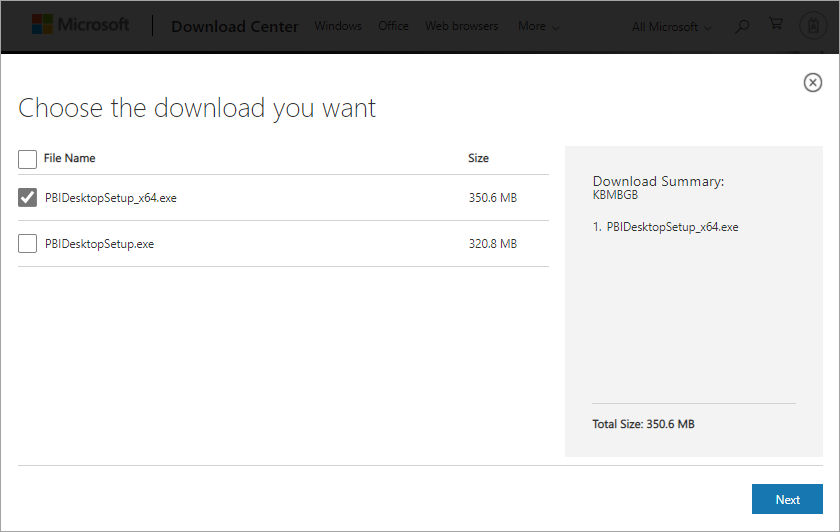
\includegraphics[width=\linewidth,height=3.9cm,keepaspectratio]{ms-learn/descargar-desktop.png}
    \fuente{Descarga de Power BI Desktop}{\urlinstalar}
    \column{0.47\textwidth}
    \small
    Con los enlaces de la diapositiva anterior:
    \begin{itemize}
      \small
      \item \textbf{Microsoft Store}: selecciona \menu{Obtener}{Get} o
        \menu{Instalar}{Install}.
      \item \textbf{Centro de descargas}: selecciona
        \menu{Descargar}{Download}, marca
        \texttt{PBIDesktopSetup\_x64.exe} (64 bits), como en la captura, y
        ejecuta el instalador.
    \end{itemize}
    \begin{alertblock}{Requisitos mínimos}
      \footnotesize Windows 10 o posterior, de 64 bits; 2 GB de RAM (se
      recomiendan 4 GB); pantalla de al menos 1440x900. \textbf{No hay
      versión para Mac}: usa un computador con Windows.
      Para saber si es de 64 bits, busca \textit{Información del
      sistema} en Inicio y mira \textit{Tipo de sistema}.
    \end{alertblock}
  \end{columns}
\end{frame}

\begin{frame}[t]{La interfaz: tres vistas}
  \begin{columns}[T,onlytextwidth]
    \column{0.46\textwidth}
    \centering
    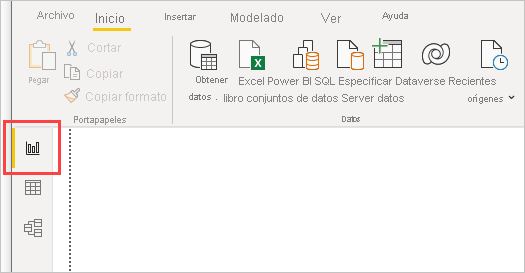
\includegraphics[width=\linewidth,height=4.0cm,keepaspectratio]{ms-learn/vistas.png}
    \fuente{Descripción general de consultas en Power BI Desktop}{\urlconsultas}
    \column{0.51\textwidth}
    \small
    Los íconos de la izquierda, de arriba abajo, cambian de vista:
    \begin{itemize}
      \small
      \item \textbf{Informe}: el lienzo donde se construyen los gráficos
        (Clase 14).
      \item \textbf{Tabla}: las filas y columnas ya cargadas, para
        revisarlas (como \texttt{df.head()}).
      \item \textbf{Modelo}: el diagrama con las tablas y sus relaciones
        (Hora 3).
    \end{itemize}
    \footnotesize Puede que veas un cuarto ícono, \textbf{Vista de
    consultas DAX}: hoy no lo usamos. El Editor de Power Query tampoco es
    una vista: es una ventana aparte (Hora 2).
  \end{columns}
\end{frame}

\begin{frame}[t]{Un archivo nuevo, todavía vacío}
  \begin{columns}[T,onlytextwidth]
    \column{0.6\textwidth}
    \centering
    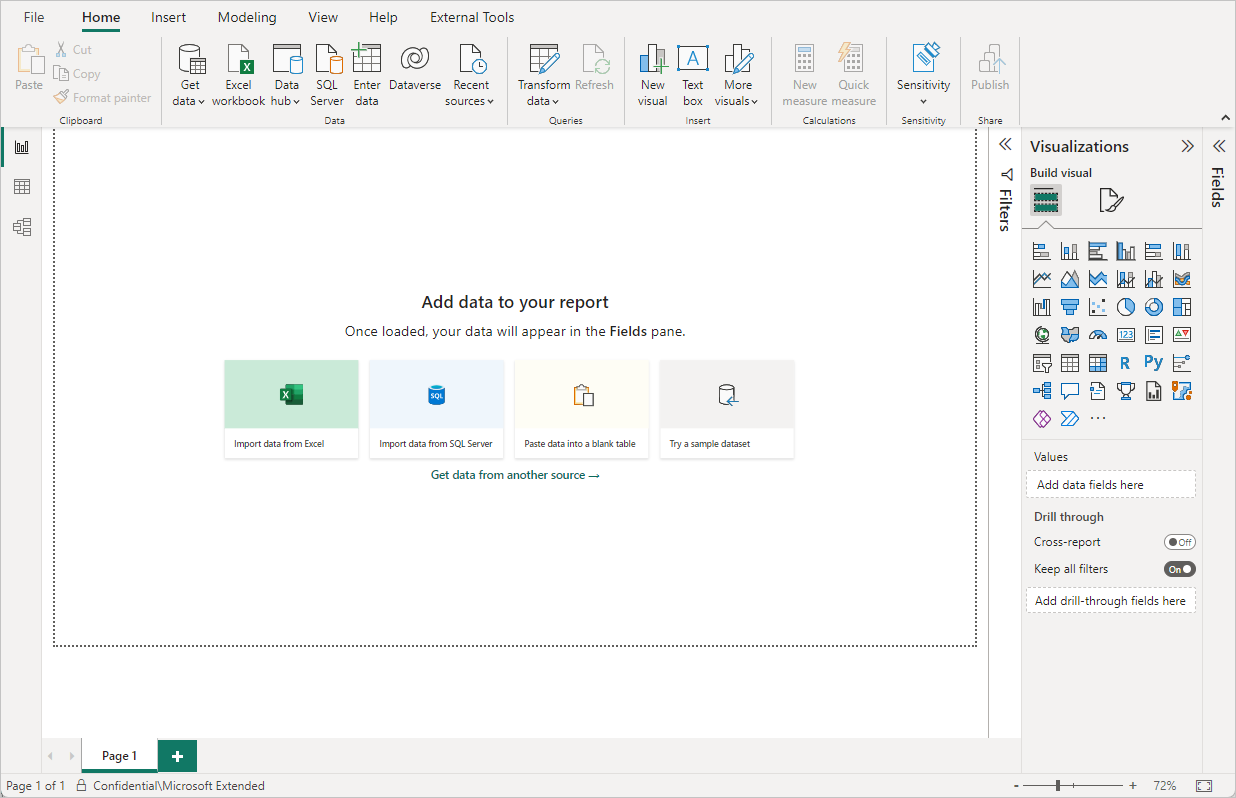
\includegraphics[width=\linewidth,height=4.7cm,keepaspectratio]{ms-learn/lienzo-en-blanco.png}
    \fuente{Inicio rápido: Conexión a datos en Power BI Escritorio}{\urlconectar}
    \column{0.37\textwidth}
    \small
    Así se ve Power BI Desktop al abrirlo:
    \begin{itemize}
      \small
      \item Arriba, la \textbf{cinta} con las pestañas.
      \item Al centro, el \textbf{lienzo} del informe.
      \item A la derecha, los paneles \textbf{Visualizaciones} y
        \textbf{Datos} (antes llamado Campos), que estarán vacíos hasta
        que cargues datos.
    \end{itemize}
  \end{columns}
\end{frame}

\begin{frame}[t]{Nuestros datos: \texttt{gimnasio\_vitalis.xlsx}}
  \small
  El mismo gimnasio del Módulo 2, ahora con 300 socios, un año de pagos y
  de entradas, y una columna nueva: \texttt{sexo}. Los 50 socios originales
  conservan sus datos.
  \vspace{0.15cm}

  \footnotesize
  \renewcommand{\arraystretch}{1.12}
  \begin{tabular}{@{}l L{6.0cm} r l@{}}
    \toprule
    \textbf{Hoja} & \textbf{Una fila es\ldots} & \textbf{Filas} & \textbf{Tipo de tabla} \\
    \midrule
    \texttt{Socios} & un socio, con su lugar de residencia (y errores puestos a propósito) & 306 & dimensión \\
    \texttt{Planes} & un plan: Mensual, Trimestral, Semestral, Anual & 4 & dimensión \\
    \texttt{Sedes} & una sede: ciudad, fecha de apertura y coordenadas & 5 & dimensión \\
    \texttt{Pagos} & un pago de un socio, de sep 2025 a sep 2026 & 1396 & hechos \\
    \texttt{Asistencias} & una entrada de un socio a una sede & 17083 & hechos \\
    \bottomrule
  \end{tabular}

  \vspace{0.2cm}
  \small La última columna es el tema de la Hora 3. Por ahora, basta con
  notar que hay tablas que \textbf{describen} (quién, qué, dónde) y tablas
  que \textbf{registran eventos} (cada pago, cada entrada).
\end{frame}

\begin{frame}[t]{\npaso{1}\; Obtener datos}
  \begin{columns}[T,onlytextwidth]
    \column{0.5\textwidth}
    \centering
    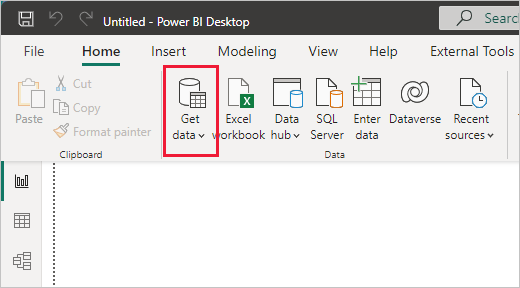
\includegraphics[width=\linewidth,height=4.2cm,keepaspectratio]{ms-learn/obtener-datos.png}
    \fuente{Inicio rápido: Conexión a datos en Power BI Escritorio}{\urlconectar}
    \column{0.47\textwidth}
    \small
    \begin{enumerate}
      \small
      \item Abre Power BI Desktop y cierra la ventana de bienvenida.
      \item En la cinta \menu{Inicio}{Home}, selecciona \menu{Obtener
        datos}{Get data}.
      \item Se despliega un menú con los orígenes más comunes. Elige
        \menu{Más\ldots}{More\ldots} al final de la lista para abrir la
        ventana completa.
    \end{enumerate}
    \footnotesize Atajo: el botón \menu{Libro de Excel}{Excel workbook},
    junto a Obtener datos, te lleva directo a elegir el archivo.
    \vspace{0.05cm}
    \footnotesize En pandas era \texttt{pd.read\_excel()}.
  \end{columns}
\end{frame}

\begin{frame}[t]{\npaso{2}\; Elegir el conector de Excel}
  \begin{columns}[T,onlytextwidth]
    \column{0.42\textwidth}
    \centering
    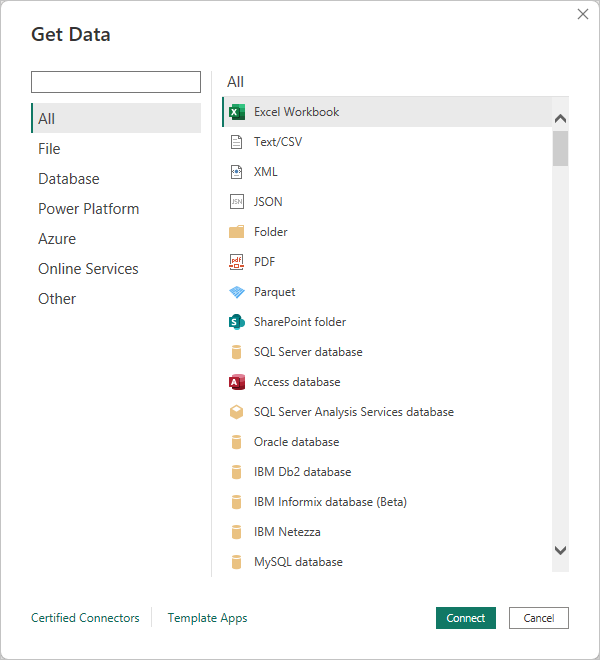
\includegraphics[width=\linewidth,height=4.7cm,keepaspectratio]{ms-learn/ventana-obtener-datos.png}
    \fuente{Inicio rápido: Conexión a datos en Power BI Escritorio}{\urlconectar}
    \column{0.55\textwidth}
    \small
    \begin{enumerate}
      \small
      \item En la ventana \menu{Obtener datos}{Get Data}, elige \menu{Libro
        de Excel}{Excel Workbook} y selecciona \menu{Conectar}{Connect}.
      \item Busca \texttt{gimnasio\_vitalis.xlsx} en tu computador y
        selecciona \menu{Abrir}{Open}.
    \end{enumerate}
    \vspace{0.1cm}
    \small Cada opción de esta lista es un \textbf{conector}: la parte de
    Power BI que sabe leer un tipo de archivo. Un CSV se abre igual, con el
    conector \menu{Texto o CSV}{Text/CSV}.
  \end{columns}
\end{frame}

\begin{frame}[t]{\npaso{3}\; El Navegador: elegir las hojas}
  \begin{columns}[T,onlytextwidth]
    \column{0.48\textwidth}
    \centering
    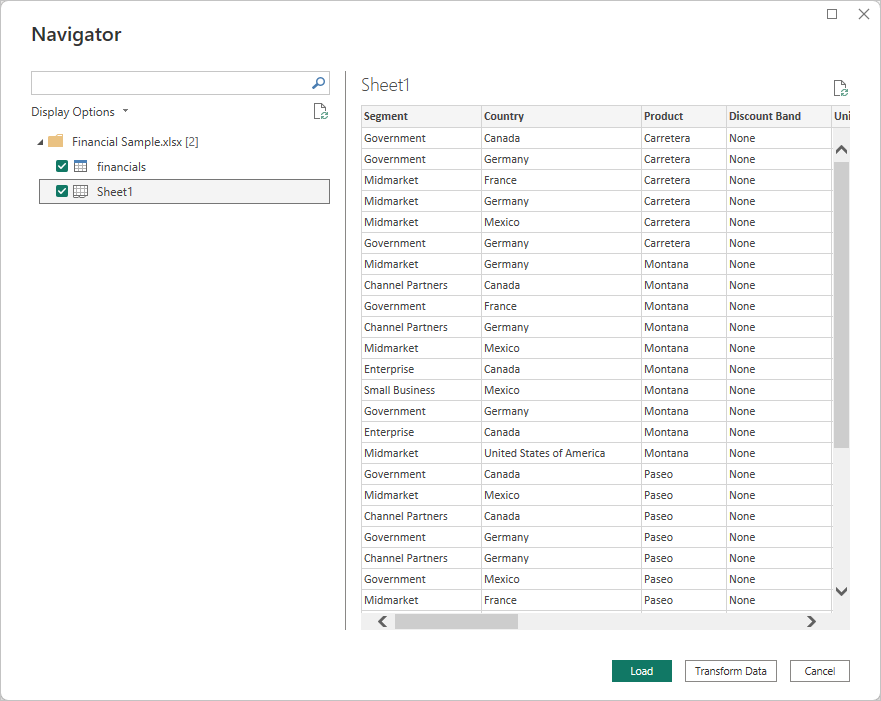
\includegraphics[width=\linewidth,height=4.7cm,keepaspectratio]{ms-learn/navegador.png}
    \fuente{Inicio rápido: Conexión a datos en Power BI Escritorio}{\urlconectar}
    \column{0.49\textwidth}
    \small
    \begin{enumerate}
      \small
      \item Marca las cinco hojas: \texttt{Socios}, \texttt{Planes},
        \texttt{Sedes}, \texttt{Pagos} y \texttt{Asistencias}.
      \item Al seleccionar una, a la derecha ves sus primeras filas.
      \item Selecciona \menu{Transformar datos}{Transform Data}, no
        \menu{Cargar}{Load}. Se abre una ventana nueva: el Editor de Power
        Query.
    \end{enumerate}
    \begin{alertblock}{¿Por qué no Cargar?}
      \footnotesize \textbf{Cargar} mete los datos al modelo tal como
      están, con duplicados y errores. \textbf{Transformar datos} te deja
      limpiarlos antes.
    \end{alertblock}
  \end{columns}
\end{frame}

% ============================================================
\section{Hora 2: Power Query}
% ============================================================
\begin{frame}[t]{¿Qué es Power Query?}
  \begin{columns}[T,onlytextwidth]
    \column{0.52\textwidth}
    \small
    Es el editor donde limpias y transformas los datos \textbf{antes} de
    que lleguen al modelo. Funciona como el pipeline de la Clase 8:
    \begin{itemize}
      \small
      \item Cada clic que das queda guardado como un \textbf{paso}, en
        orden.
      \item El archivo original \textbf{no cambia}: Power Query cambia su
        vista de los datos, como nunca editábamos el CSV crudo.
      \item Si el Excel se actualiza, \menu{Actualizar}{Refresh} repite
        todos los pasos solos.
    \end{itemize}
    \column{0.45\textwidth}
    \centering
    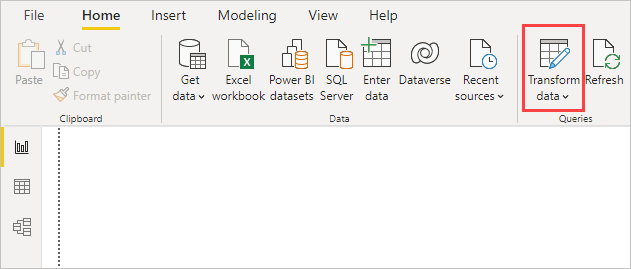
\includegraphics[width=\linewidth,height=3.4cm,keepaspectratio]{ms-learn/boton-transformar-datos.png}
    \fuente{Descripción general de consultas en Power BI Desktop}{\urlconsultas}
    \vspace{0.1cm}
    \raggedright\footnotesize Si ya cargaste los datos, vuelves al editor
    cuando quieras con \menu{Transformar datos}{Transform data} en la
    cinta \menu{Inicio}{Home}.
  \end{columns}
\end{frame}

\begin{frame}[t]{Las cinco zonas del Editor de Power Query}
  \begin{columns}[T,onlytextwidth]
    \column{0.6\textwidth}
    \centering
    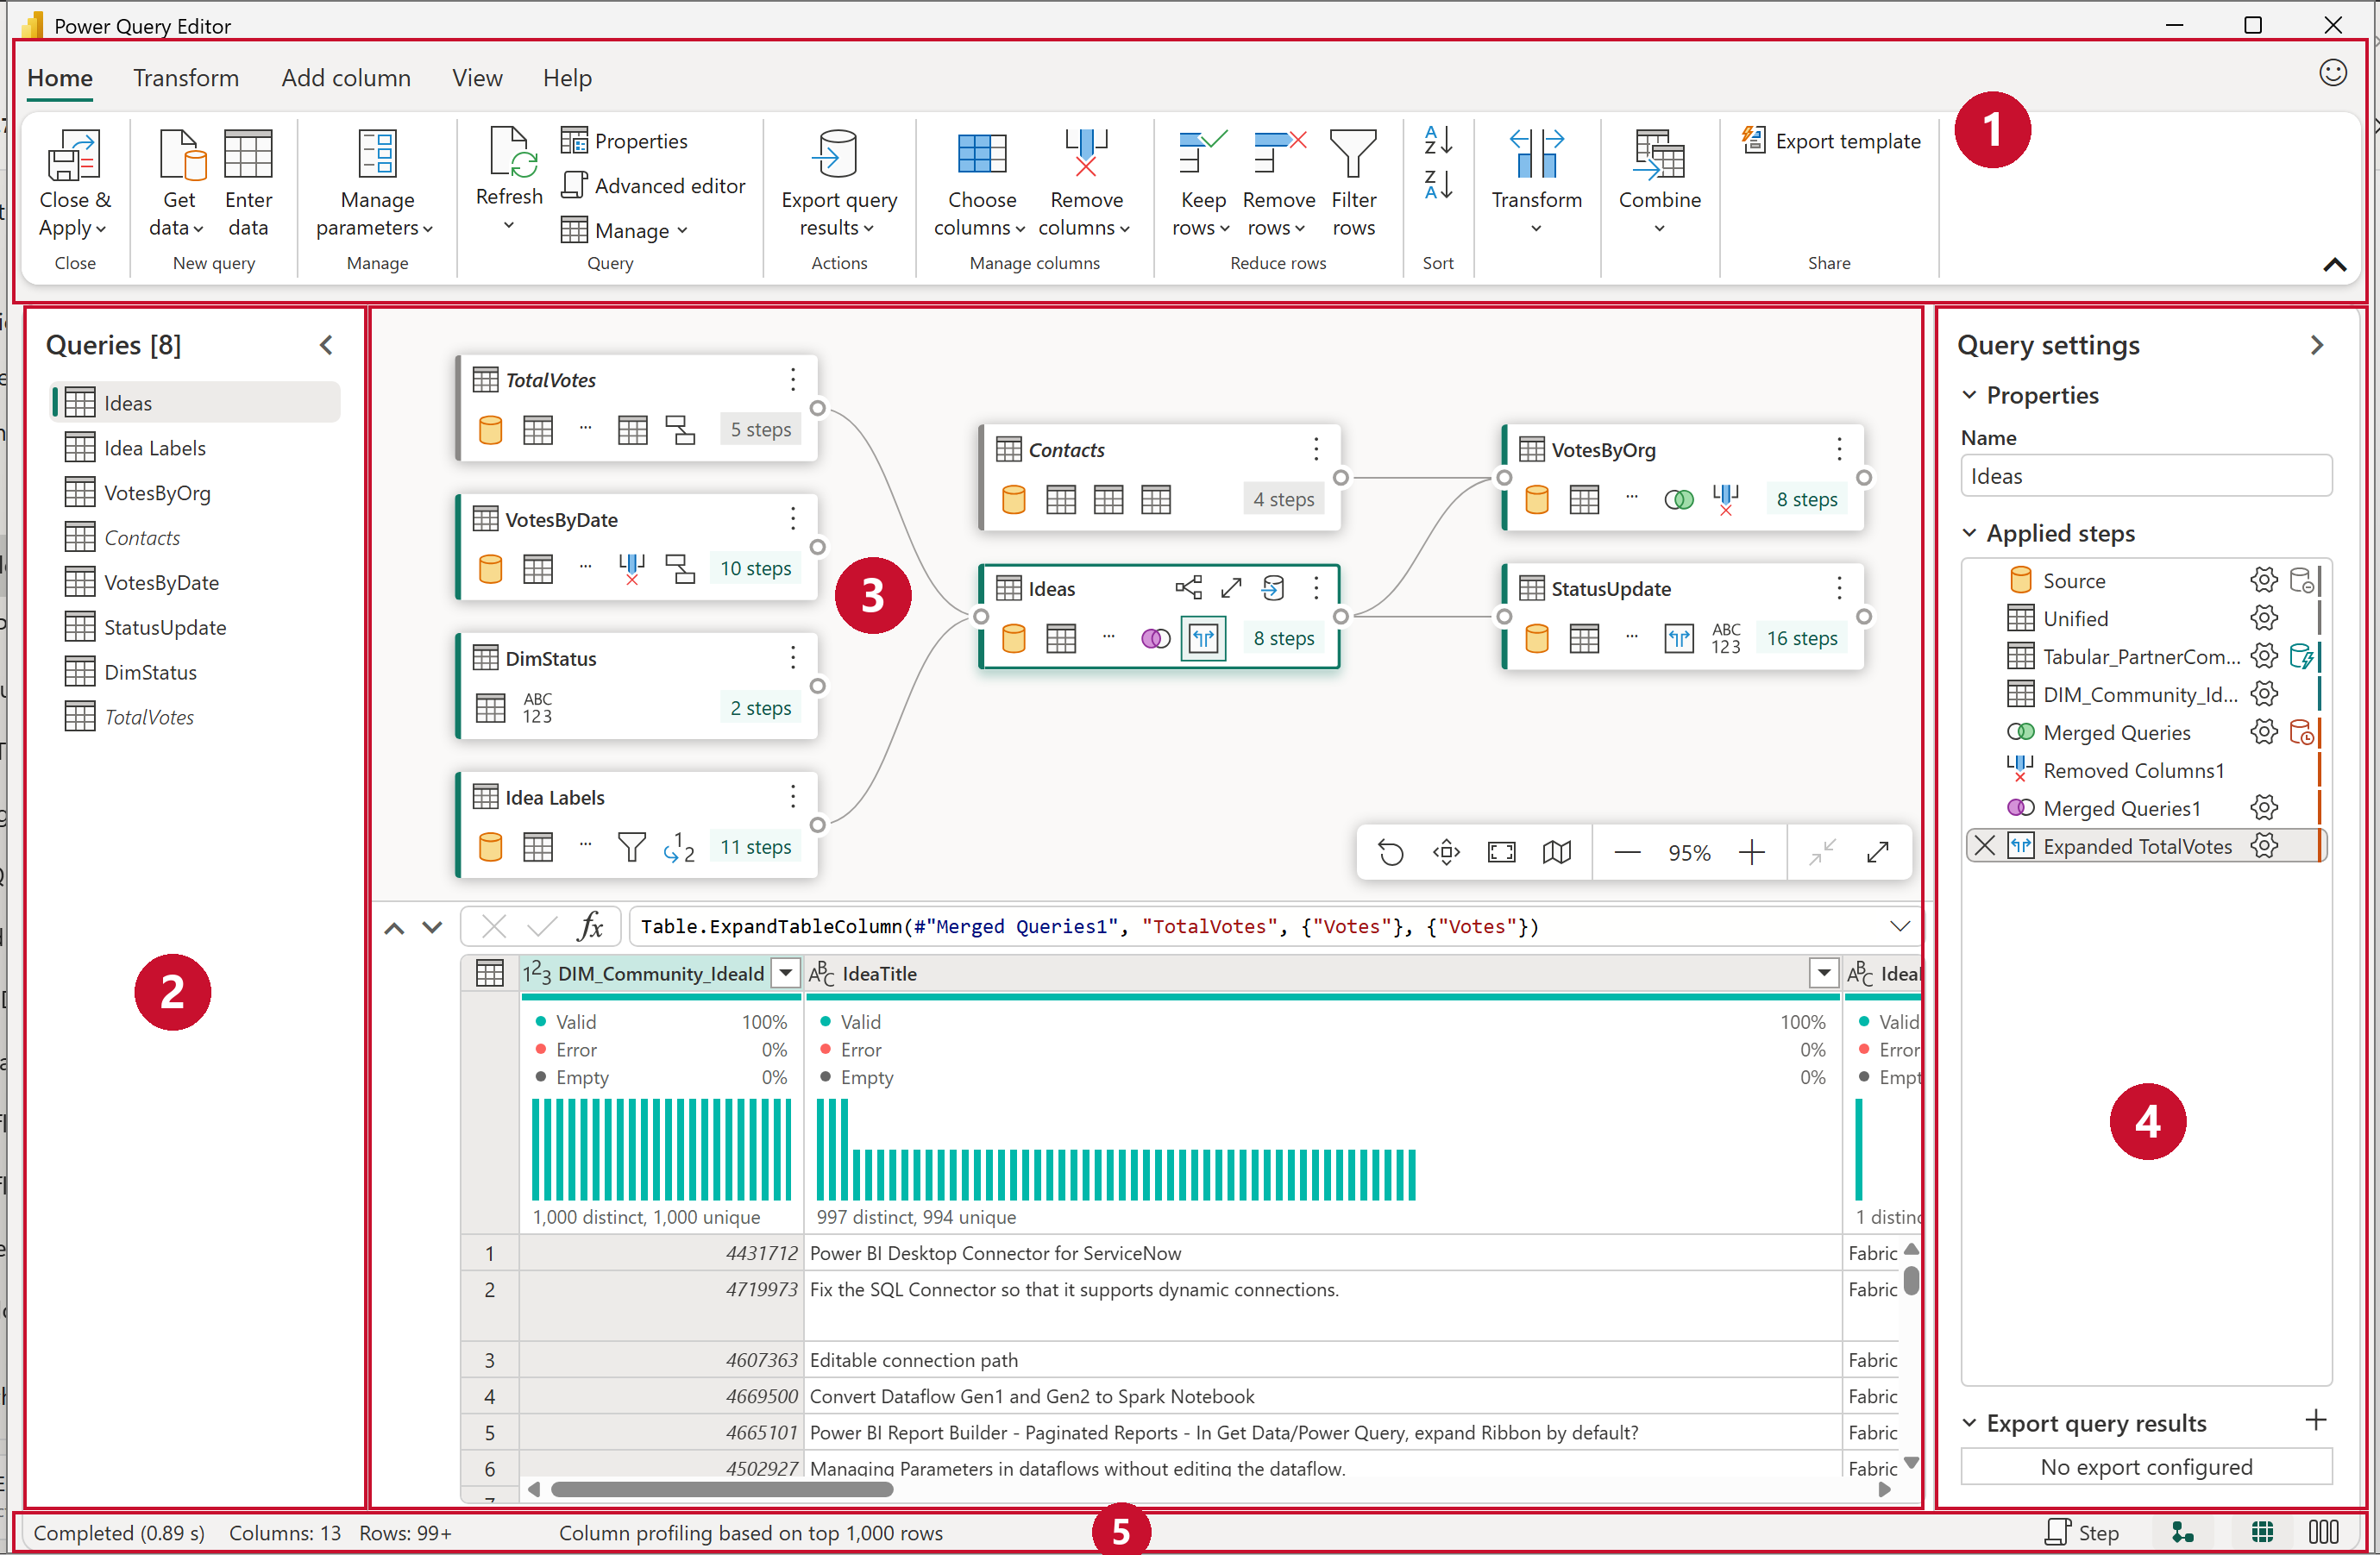
\includegraphics[width=\linewidth,height=4.9cm,keepaspectratio]{ms-learn/editor-zonas.png}
    \fuente{Descripción general de consultas en Power BI Desktop}{\urlconsultas}
    \column{0.37\textwidth}
    \footnotesize
    \begin{enumerate}
      \footnotesize
      \item \textbf{Cinta de opciones}: las pestañas con todas las
        transformaciones.
      \item \textbf{Panel de consultas}: una consulta por cada hoja que
        trajiste.
      \item \textbf{Vista actual}: la vista previa de los datos.
      \item \textbf{Configuración de consulta}: el nombre y la lista de
        \textbf{pasos aplicados}.
      \item \textbf{Barra de estado}: cuántas filas y columnas tiene la
        consulta.
    \end{enumerate}
  \end{columns}
\end{frame}

\begin{frame}[t]{Las pestañas que más vas a usar}
  \small
  \textbf{Transformar} (Transform) cambia una columna que ya existe:
  tipo de dato, reemplazar valores, formato de texto, dividir columnas.
  \begin{center}
    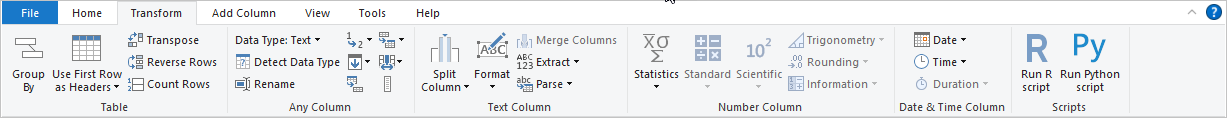
\includegraphics[width=0.96\textwidth]{ms-learn/cinta-transformar.png}
  \end{center}
  \textbf{Agregar columna} (Add Column) crea una columna nueva a partir de
  otras: columna personalizada, columna condicional.
  \begin{center}
    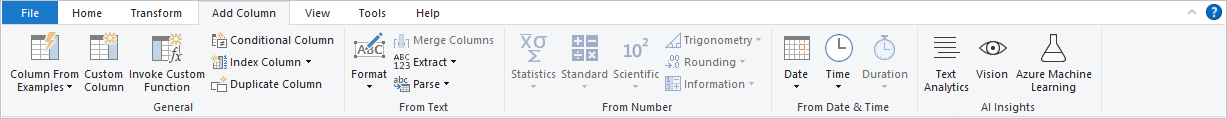
\includegraphics[width=0.96\textwidth]{ms-learn/cinta-agregar-columna.png}
  \end{center}
  \fuente{Descripción general de consultas en Power BI Desktop}{\urlconsultas}
  \vspace{0.05cm}
  \footnotesize La pestaña \menu{Inicio}{Home} tiene las tareas comunes
  (quitar filas, combinar consultas, cerrar y aplicar), y \menu{Vista}{View}
  las herramientas de perfil de columnas del paso siguiente.
\end{frame}

\begin{frame}[t]{\npaso{4}\; Mira la calidad de cada columna}
  \begin{columns}[T,onlytextwidth]
    \column{0.55\textwidth}
    \centering
    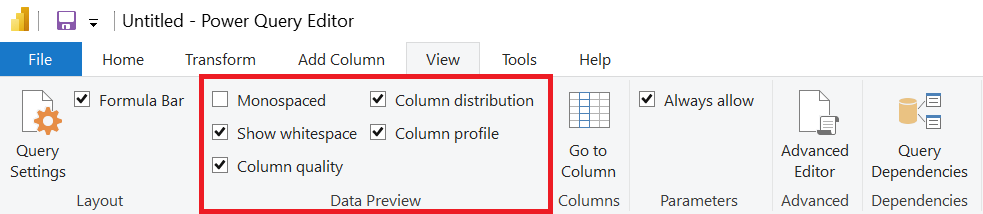
\includegraphics[width=\linewidth,height=2.6cm,keepaspectratio]{ms-learn/vista-perfilado.png}
    \fuente{Uso de las herramientas de generación de perfiles de datos}{https://learn.microsoft.com/es-es/power-query/data-profiling-tools}
    \vspace{0.15cm}
    \begin{exampleblock}{En pandas (Clase 7)}
      \footnotesize Es el diagnóstico de calidad:
      \texttt{df.isna().sum()} y \texttt{value\_counts()} de cada
      columna, pero dibujado debajo de cada encabezado.
    \end{exampleblock}
    \begin{alertblock}{Solo 1000 filas}
      \footnotesize Abajo a la izquierda dice \textit{Generación de
      perfiles de columna basada en las 1000 primeras filas}. Haz clic ahí
      y elige el conjunto de datos completo.
    \end{alertblock}
    \column{0.42\textwidth}
    \small
    \begin{enumerate}
      \small
      \item En el panel de consultas, a la izquierda, haz clic en
        \texttt{Socios}.
      \item En la pestaña \menu{Vista}{View}, marca \menu{Calidad de
        columnas}{Column quality}, \menu{Distribución de
        columnas}{Column distribution} y \menu{Perfil de
        columna}{Column profile}.
      \item Bajo cada título de columna verás: \textbf{Válido} (dato bien
        leído), \textbf{Error} (no se pudo leer) y \textbf{Vacío} (celda
        sin dato, como un \texttt{NaN}).
    \end{enumerate}
  \end{columns}
\end{frame}

\begin{frame}[t]{El diagnóstico de la hoja \texttt{Socios}}
  \small
  Esto es lo que deberías encontrar. Cada problema se resuelve con uno de
  los pasos siguientes.
  \vspace{0.15cm}

  \footnotesize
  \renewcommand{\arraystretch}{1.15}
  \begin{tabular}{@{}L{2.3cm}L{4.0cm}L{3.0cm}L{3.3cm}@{}}
    \toprule
    \textbf{Problema} & \textbf{Qué ves} & \textbf{Paso de hoy} & \textbf{En pandas} \\
    \midrule
    Filas duplicadas & 306 filas, pero solo 300 \texttt{id\_socio} distintos & \npaso{5} Quitar duplicados & \texttt{drop\_duplicates()} \\
    Tipo incorrecto & \texttt{telefono} es un número; las fechas pueden traer hora & \npaso{6} Tipo de datos & \texttt{astype(str)} \\
    Texto sucio & nombres con espacios sobrantes o en minúsculas & \npaso{7} Recortar y formato & \texttt{str.strip()} \texttt{.str.title()} \\
    Inconsistencias & \texttt{sexo} escrito de 12 formas, y 10 celdas vacías & \npaso{8}\npaso{9} Reemplazar valores & \texttt{replace()}, \texttt{fillna()} \\
    Dato que falta & no hay columna de edad, solo la fecha de nacimiento & \npaso{10}\npaso{11} Columnas nuevas & resta de fechas, \texttt{pd.cut} \\
    \bottomrule
  \end{tabular}
\end{frame}

\begin{frame}[t]{\npaso{5}\; Quitar duplicados}
  \begin{columns}[T,onlytextwidth]
    \column{0.55\textwidth}
    \centering
    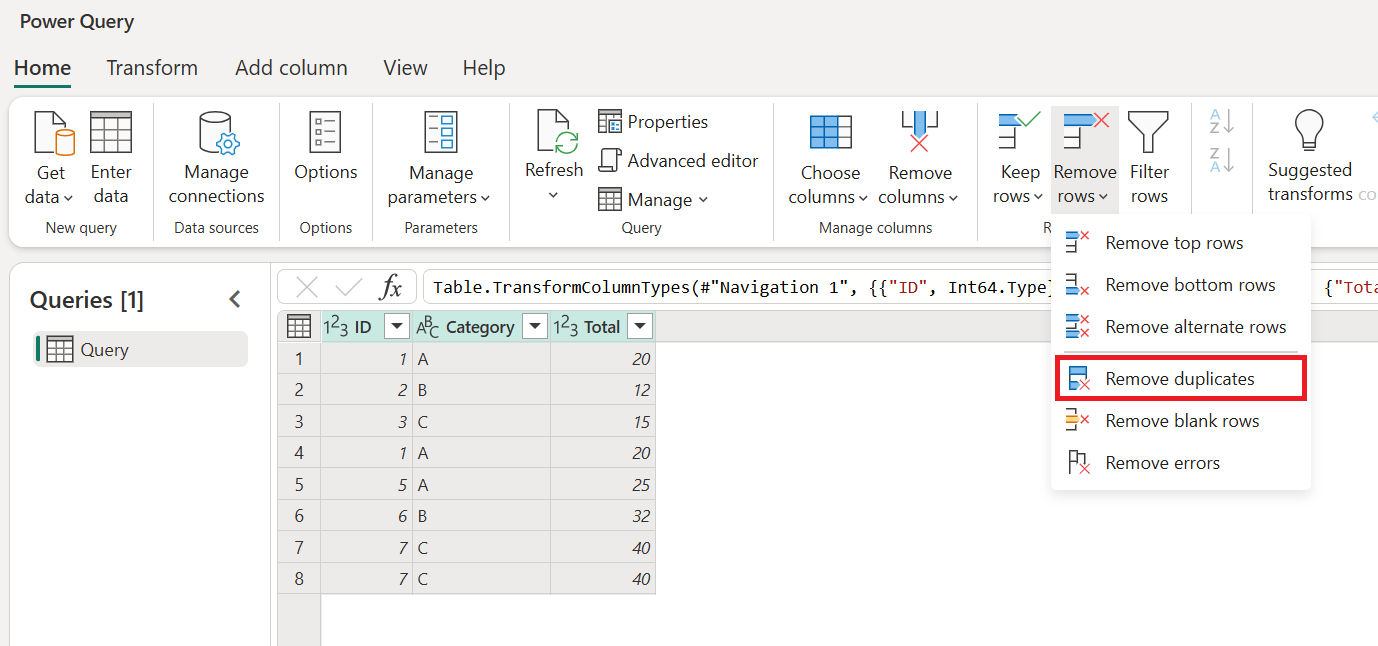
\includegraphics[width=\linewidth,height=3.4cm,keepaspectratio]{ms-learn/quitar-duplicados.png}
    \fuente{Trabajar con valores duplicados}{https://learn.microsoft.com/es-es/power-query/working-with-duplicates}
    \vspace{0.15cm}
    \begin{exampleblock}{En pandas (Clase 8)}
      \footnotesize \texttt{socios.drop\_duplicates(subset="id\_socio")}
    \end{exampleblock}
    \column{0.42\textwidth}
    \small
    \begin{enumerate}
      \small
      \item Selecciona la columna \texttt{id\_socio} (clic en su
        encabezado).
      \item En \menu{Inicio}{Home}, abre \menu{Quitar filas}{Remove rows}
        y elige \menu{Quitar duplicados}{Remove duplicates}.
      \item Mira la barra de estado, abajo a la izquierda: de 306 filas
        pasas a \textbf{300}.
    \end{enumerate}
    \small Va primero porque \texttt{id\_socio} es la \textbf{llave} de
    \texttt{Socios} (la columna que identifica a cada socio) y debe ser
    única: si se repite, la relación de la Hora 3 no se puede crear.
  \end{columns}
\end{frame}

\begin{frame}[t]{\npaso{6}\; Tipos de datos correctos}
  \small
  El ícono a la izquierda de cada título de columna muestra su tipo
  (número, texto, fecha\ldots). Haz clic en él para cambiarlo:
  \begin{center}
    
\includegraphics[width=0.92\textwidth]{ms-learn/iconos-tipos-datos.png}
    \fuente{Tipos de datos en Power Query}{https://learn.microsoft.com/es-es/power-query/data-types}
  \end{center}
  \vspace{-0.1cm}
  \begin{columns}[T,onlytextwidth]
    \column{0.55\textwidth}
    \begin{enumerate}
      \footnotesize
      \item \texttt{telefono} $\Rightarrow$ \menu{Texto}{Text}: un teléfono
        no es una cantidad que se sume.
      \item Fechas: si su ícono es un calendario con reloj y los valores
        traen una hora (12:00:00 a.\,m.), cámbialas a \menu{Fecha}{Date}.
        Son \texttt{fecha\_nacimiento} y \texttt{fecha\_inscripcion} aquí,
        y también \texttt{Pagos[fecha\_pago]} y \texttt{Asistencias[fecha]}.
      \item Si aparece la pregunta \textit{Cambiar tipo de columna}, elige
        \menu{Reemplazar actual}{Replace current}: corrige el paso de tipo
        que ya existe en vez de agregar otro.
    \end{enumerate}
    \column{0.42\textwidth}
    \begin{alertblock}{Revisa el paso automático}
      \footnotesize Al traer los datos, Power Query adivina los tipos y
      agrega solo un paso \textbf{Tipo cambiado} (Changed Type). Casi
      siempre acierta, pero no con teléfonos, códigos ni fechas.
    \end{alertblock}
  \end{columns}
\end{frame}

\begin{frame}[t]{\npaso{7}\; Limpiar el texto de \texttt{nombre}}
  \begin{columns}[T,onlytextwidth]
    \column{0.4\textwidth}
    \centering
    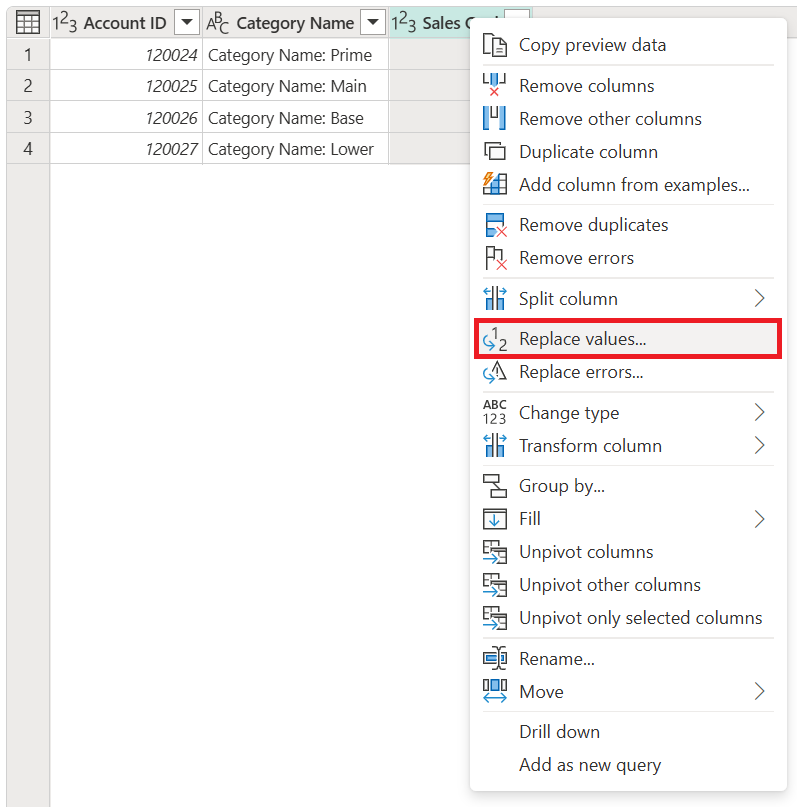
\includegraphics[width=\linewidth,height=4.8cm,keepaspectratio]{ms-learn/menu-columna.png}
    \fuente{Reemplazar valores y errores}{https://learn.microsoft.com/es-es/power-query/replace-values}
    \column{0.57\textwidth}
    \small
    Clic derecho sobre el encabezado de una columna abre este menú: casi
    todas las transformaciones están también aquí.
    \begin{enumerate}
      \small
      \item Clic derecho en \texttt{nombre} $>$ \menu{Transformar}{Transform}
        $>$ \menu{Recortar}{Trim}: quita los espacios al inicio y al final.
      \item De nuevo \menu{Transformar}{Transform} $>$ \menu{Poner En
        Mayúsculas Cada Palabra}{Capitalize Each Word}.
    \end{enumerate}
    \begin{exampleblock}{En pandas (Clase 8)}
      \footnotesize \texttt{socios["nombre"].str.strip().str.title()}
    \end{exampleblock}
    \footnotesize 24 nombres cambian con estos dos pasos.
  \end{columns}
\end{frame}

\begin{frame}[t]{\npaso{8}\; Unificar \texttt{sexo}: primero, el mismo formato}
  \small
  La columna tiene 12 formas de escribir dos valores. Antes de reemplazar,
  conviene reducir las variantes con dos transformaciones de formato:
  \vspace{0.2cm}
  \begin{center}
  \begin{tikzpicture}[
    col/.style={draw=esumerNavy!50,fill=white,rounded corners=2pt,text width=2.6cm,
                align=center,font=\scriptsize\ttfamily,inner sep=4pt},
    tit/.style={font=\bfseries\scriptsize,text=esumerNavy,align=center,text width=3.2cm},
    flecha/.style={-{Stealth[length=2.2mm]},line width=0.9pt,color=esumerOrange},
  ]
    \node[col] (a) at (0,0) {"F" " F" "f"\\ "femenino" "FEMENINO"\\ "Femenino"\\[3pt]
                            "M" "M " "m"\\ "masculino" "MASCULINO"\\ "Masculino"\\[3pt] null};
    \node[col] (b) at (5,0) {"F"\\ "FEMENINO"\\[3pt] "M"\\ "MASCULINO"\\[3pt] null};
    \node[col] (c) at (10,0) {"FEMENINO"\\[3pt] "MASCULINO"\\[3pt] null};
    \node[tit, above=0.15cm of a] {Valores en el Excel};
    \node[tit, above=0.15cm of b] {Tras Recortar y MAYÚSCULAS};
    \node[tit, above=0.15cm of c] {Tras el paso 9};
    \draw[flecha] (a) -- node[above,font=\scriptsize,text=black,align=center]{Recortar\\MAYÚSCULAS} (b);
    \draw[flecha] (b) -- node[above,font=\scriptsize,text=black,align=center]{Reemplazar\\valores} (c);
  \end{tikzpicture}
  \end{center}
  \vspace{0.1cm}
  \footnotesize
  \begin{enumerate}
    \footnotesize
    \item Clic derecho en el título \texttt{sexo} $>$
      \menu{Transformar}{Transform} $>$ \menu{Recortar}{Trim}.
    \item De nuevo: \menu{Transformar}{Transform} $>$
      \menu{MAYÚSCULAS}{UPPERCASE}.
  \end{enumerate}
  \texttt{null} es como Power Query muestra una celda vacía (el
  \texttt{NaN} de pandas). Lo resolvemos en el paso 9.
\end{frame}

\begin{frame}[t]{\npaso{9}\; Reemplazar valores, con una casilla clave}
  \begin{columns}[T,onlytextwidth]
    \column{0.52\textwidth}
    \small
    Clic derecho en \texttt{sexo} $>$ \menu{Reemplazar valores}{Replace
    values}. Llena los dos campos y repite tres veces:
    \vspace{0.1cm}

    \footnotesize
    \begin{tabular}{@{}ll@{}}
      \toprule
      \textbf{Valor que buscar} & \textbf{Reemplazar con} \\
      \midrule
      \texttt{F} & \texttt{FEMENINO} \\
      \texttt{M} & \texttt{MASCULINO} \\
      \texttt{null} & \texttt{NO INFORMADO} \\
      \bottomrule
    \end{tabular}

    \vspace{0.15cm}
    \footnotesize En el tercero escribe la palabra \texttt{null}, en
    minúsculas: así se buscan las celdas vacías.\\[3pt]
    \small Al final, clic derecho $>$ \menu{Transformar}{Transform} $>$
    \menu{Poner En Mayúsculas Cada Palabra}{Capitalize Each Word}. Debes
    obtener \textbf{145 Femenino, 146 Masculino y 9 No Informado}.
    \column{0.45\textwidth}
    \begin{alertblock}{Marca ``Coincidir con todo el contenido de la celda''}
      \footnotesize En columnas de texto, Reemplazar valores cambia
      \textbf{cada aparición} del texto, aunque esté dentro de otra
      palabra: la F de \texttt{FEMENINO} también se reemplazaría, y
      quedaría \texttt{FEMENINOEMENINO}. Abre \menu{Opciones
      avanzadas}{Advanced options} y activa esa casilla en los dos
      primeros reemplazos.
    \end{alertblock}
    \begin{exampleblock}{En pandas (Clase 8)}
      \footnotesize \texttt{.replace(\{"F": "FEMENINO"\})} reemplaza el valor
      completo; \texttt{.str.replace()}, en cambio, se comporta como Power
      Query sin la casilla.
    \end{exampleblock}
  \end{columns}
\end{frame}

\begin{frame}[t]{\npaso{10}\; Columna personalizada: la edad}
  \begin{columns}[T,onlytextwidth]
    \column{0.44\textwidth}
    \centering
    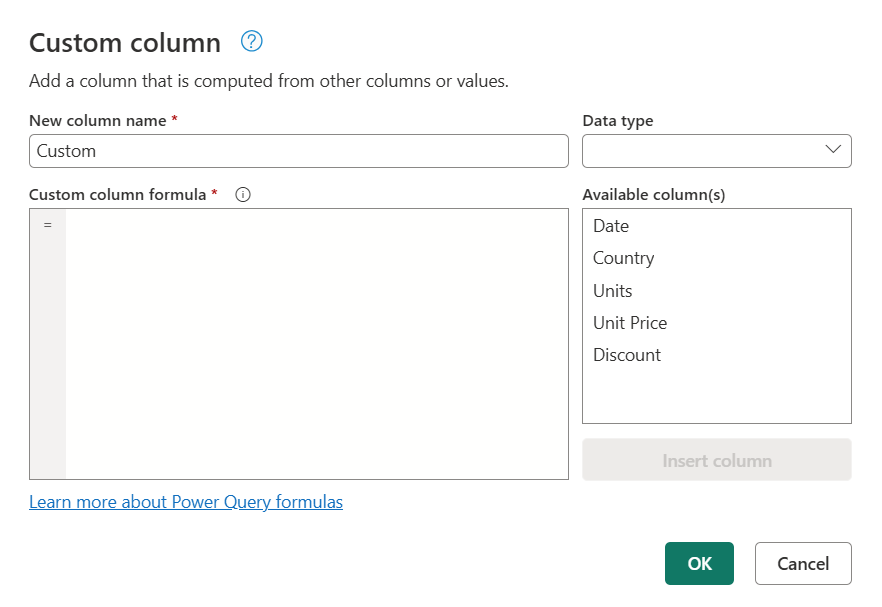
\includegraphics[width=\linewidth,height=2.9cm,keepaspectratio]{ms-learn/ventana-columna-personalizada.png}
    \fuente{Adición de una columna personalizada}{https://learn.microsoft.com/es-es/power-query/add-custom-column}
    \vspace{0.05cm}
    \begin{exampleblock}{Cómo se lee la fórmula}
      \scriptsize \texttt{\#date(2026, 9, 30)} es la fecha de corte. Al
      restarle la fecha de nacimiento queda el tiempo vivido;
      \texttt{Duration.Days} lo pasa a días, \texttt{/ 365.25} a años (el
      ,25 por los bisiestos) y \texttt{Number.RoundDown} quita los
      decimales.
    \end{exampleblock}
    \column{0.53\textwidth}
    \footnotesize
    \begin{enumerate}
      \footnotesize
      \item \menu{Agregar columna}{Add Column} $>$ \menu{Columna
        personalizada}{Custom column}.
      \item En el nombre de la columna nueva escribe \texttt{edad}.
      \item En la fórmula escribe lo siguiente. Para insertar
        \texttt{[fecha\_nacimiento]}, haz doble clic en ella en la lista de
        columnas disponibles.
    \end{enumerate}
    \vspace{-0.15cm}
    \codigo{Number.RoundDown(\\
      \hspace*{1em}Duration.Days(\\
      \hspace*{2em}\#date(2026, 9, 30) - [fecha\_nacimiento]\\
      \hspace*{1em}) / 365.25\\
      )}
    \begin{enumerate}
      \footnotesize
      \setcounter{enumi}{3}
      \item Cambia el tipo de \texttt{edad} a \menu{Número entero}{Whole
        Number}. Debe ir de 16 a 69 años.
    \end{enumerate}
    \scriptsize Cópiala tal cual: M distingue mayúsculas. Si da error,
    revisa que \texttt{fecha\_nacimiento} sea de tipo Fecha (paso 6).
  \end{columns}
\end{frame}

\begin{frame}[t]{\npaso{11}\; Columna condicional: el grupo de edad}
  \begin{center}
    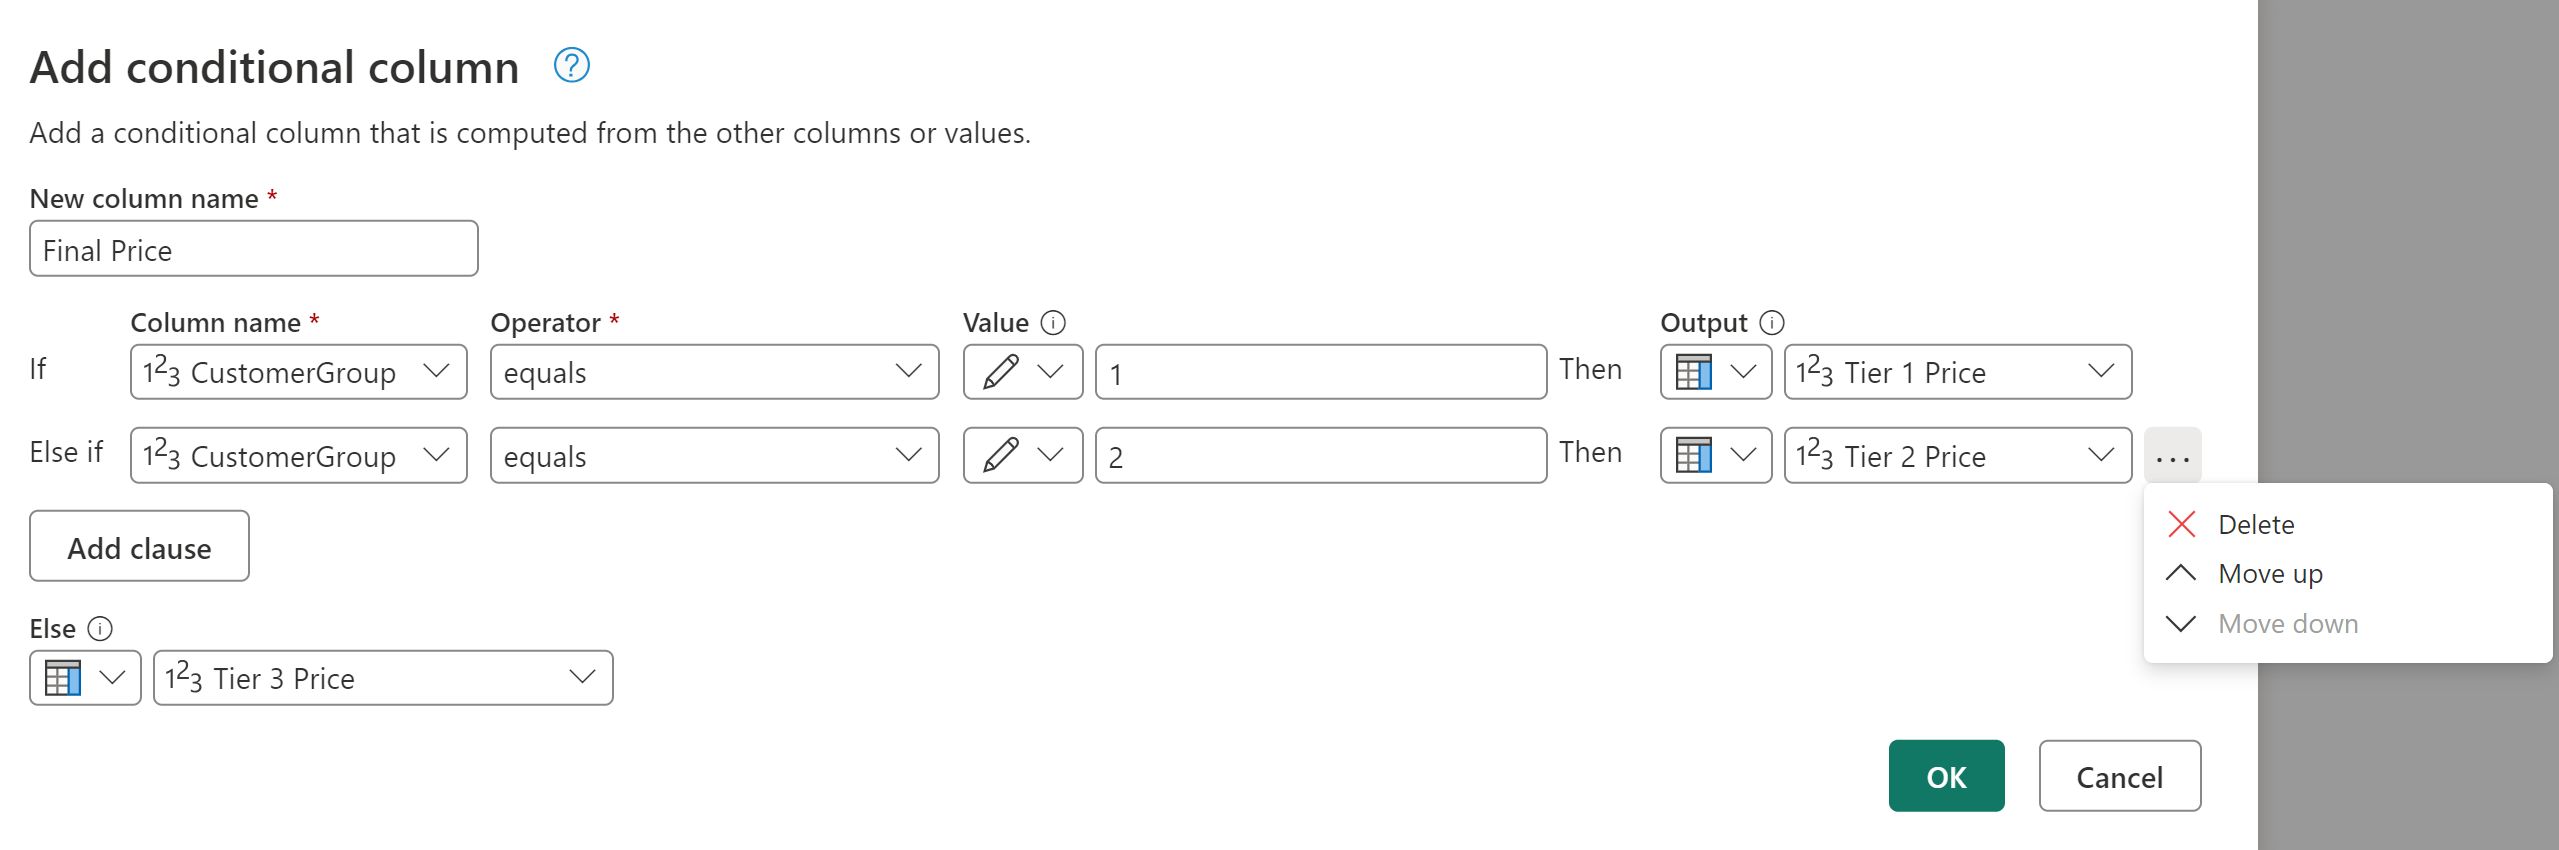
\includegraphics[width=0.86\textwidth,height=2.2cm,keepaspectratio]{ms-learn/ventana-columna-condicional.png}
    \fuente{Agregar columna condicional}{https://learn.microsoft.com/es-es/power-query/add-conditional-column}
  \end{center}
  \vspace{-0.1cm}
  \begin{columns}[T,onlytextwidth]
    \column{0.6\textwidth}
    \footnotesize
    \menu{Agregar columna}{Add Column} $>$ \menu{Columna
    condicional}{Conditional column}. Nombre: \texttt{grupo\_edad}. Cada
    fila es una cláusula:
    \vspace{0.05cm}

    \scriptsize
    \begin{tabular}{@{}llll@{}}
      \toprule
      \textbf{Columna} & \textbf{Operador} & \textbf{Valor} & \textbf{Salida} \\
      \midrule
      \texttt{edad} & menor o igual que & 25 & \texttt{Joven (<=25)} \\
      \texttt{edad} & menor o igual que & 45 & \texttt{Adulto (26-45)} \\
      \bottomrule
    \end{tabular}

    \vspace{0.05cm}
    \footnotesize La segunda se agrega con \menu{Agregar
    cláusula}{Add clause}. En el último campo (\textit{Else}) escribe
    \texttt{Mayor (46+)}.
    \column{0.37\textwidth}
    \begin{alertblock}{Ponle tipo a la columna}
      \scriptsize Una columna condicional nueva no tiene tipo de datos.
      Cámbialo a \menu{Texto}{Text}, como en el paso 6.
    \end{alertblock}
    \scriptsize En pandas: \texttt{pd.cut} (Clase 8).\\
    Comprueba: 56 jóvenes, 173 adultos y 71 mayores.
  \end{columns}
\end{frame}

\begin{frame}[t]{\npaso{12}\; Combinar consultas: la sede de cada socio}
  \begin{columns}[T,onlytextwidth]
    \column{0.34\textwidth}
    \centering
    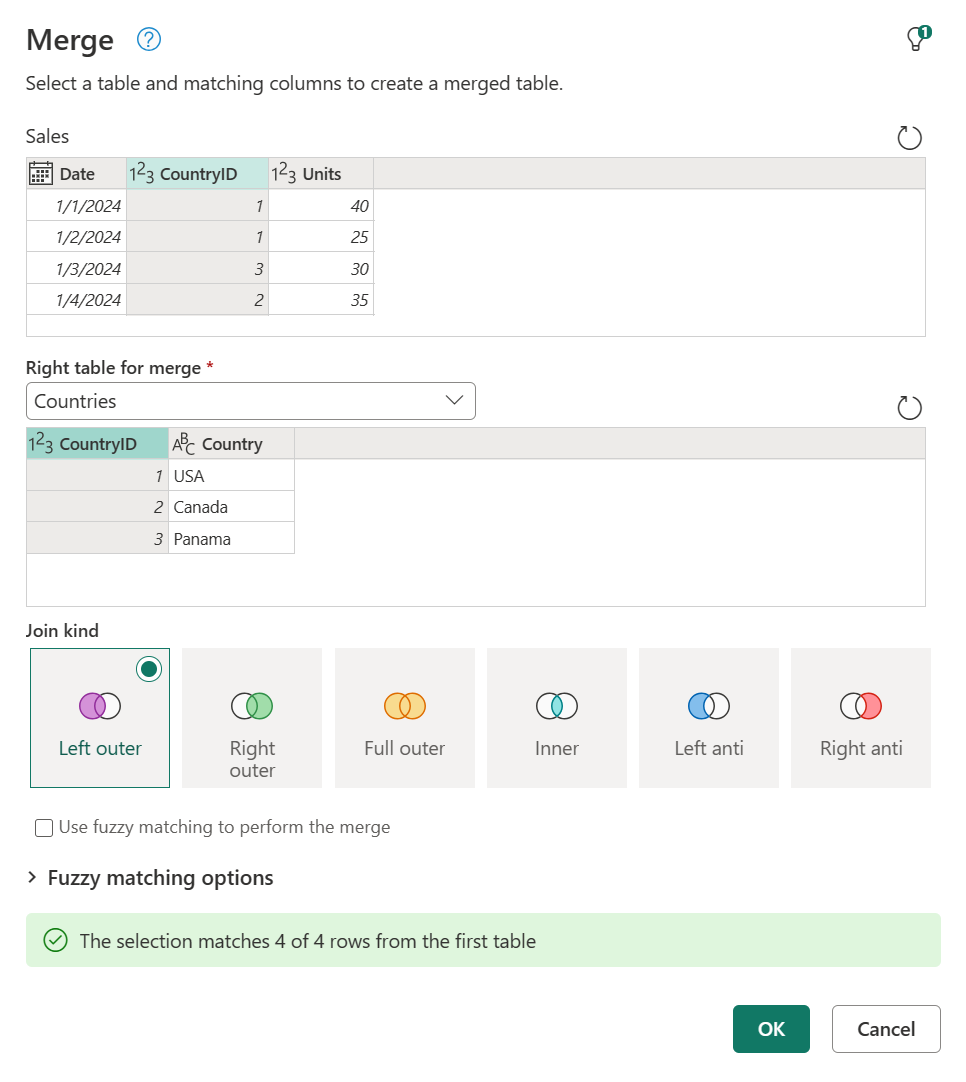
\includegraphics[width=\linewidth,height=4.6cm,keepaspectratio]{ms-learn/ventana-combinar.png}
    \fuente{Visión general de las consultas de combinación}{https://learn.microsoft.com/es-es/power-query/merge-queries-overview}
    \column{0.63\textwidth}
    \footnotesize
    \texttt{Socios} solo trae el número de su sede
    (\texttt{id\_sede\_principal}). Para traer el nombre:
    \begin{enumerate}
      \footnotesize
      \item Con \texttt{Socios} seleccionada: \menu{Inicio}{Home} $>$
        \menu{Combinar consultas}{Merge queries}.
      \item Arriba está \texttt{Socios}: haz clic en el título
        \texttt{id\_sede\_principal}. Abajo elige \texttt{Sedes} y haz clic
        en \texttt{id\_sede}.
      \item Tipo de combinación: \menu{Externa izquierda}{Left outer}.
        Acepta.
      \item Aparece una columna \texttt{Sedes} que dice \textit{Table} en
        cada fila. Haz clic en el ícono de dos flechas de su título, deja
        marcada solo \texttt{sede} y \textbf{desmarca} \menu{Usar nombre de
        columna original como prefijo}{Use original column name as prefix}.
      \item Doble clic en el título para renombrarla
        \texttt{sede\_principal}.
    \end{enumerate}
    \scriptsize En pandas: un \texttt{merge(how="left")}, como en la Clase 10.
  \end{columns}
\end{frame}

\begin{frame}[t]{¿Combinar consultas o relacionar tablas?}
  \small
  En pandas, para analizar dos tablas juntas casi siempre hacías un
  \texttt{merge}. En Power BI la regla cambia:
  \vspace{0.15cm}
  \begin{columns}[T,onlytextwidth]
    \column{0.48\textwidth}
    \begin{exampleblock}{Relaciona (Hora 3)}
      \small Cuando cada tabla describe una cosa distinta: socios, planes,
      sedes, pagos. Quedan separadas y el modelo las conecta. Es lo
      normal.
    \end{exampleblock}
    \column{0.48\textwidth}
    \begin{alertblock}{Combina (Power Query)}
      \small Cuando un dato debe ser \textbf{una columna más} de otra
      tabla, como la sede principal de cada socio, o cuando dos tablas son
      en realidad una sola.
    \end{alertblock}
  \end{columns}
  \vspace{0.2cm}
  \small ¿Por qué se llama \texttt{id\_sede\_principal} y no
  \texttt{id\_sede}? Power BI une por su cuenta las columnas que se llaman
  igual. Si uniera \texttt{Socios} con \texttt{Sedes}, un filtro por sede
  llegaría a los pagos por dos caminos distintos, y eso confunde los
  resultados (Hora 3).
\end{frame}

\begin{frame}[t]{Pasos aplicados: tu pipeline, guardado}
  \begin{columns}[T,onlytextwidth]
    \column{0.32\textwidth}
    \centering
    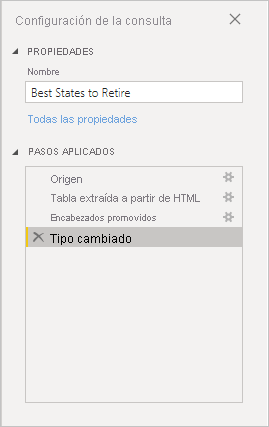
\includegraphics[width=\linewidth,height=4.8cm,keepaspectratio]{ms-learn/pasos-aplicados.png}
    \fuente{Descripción general de consultas en Power BI Desktop}{\urlconsultas}
    \column{0.65\textwidth}
    \small
    Todo lo que hiciste quedó en \textbf{Pasos aplicados} (Applied steps),
    en el panel de la derecha:
    \begin{itemize}
      \small
      \item \textbf{Clic en un paso}: ves los datos tal como estaban en
        ese momento.
      \item \textbf{Clic derecho}: cambiar el nombre, eliminar o mover el
        paso. Dale nombres que digan qué hacen, como ``Sexo unificado''.
      \item \menu{Vista}{View} $>$ \menu{Editor avanzado}{Advanced editor}
        muestra el código M de todos los pasos.
    \end{itemize}
    \begin{exampleblock}{En pandas}
      \footnotesize Es el notebook de la Clase 8: una celda por paso,
      ejecutadas en orden, sin editar nunca el archivo original.
    \end{exampleblock}
  \end{columns}
\end{frame}

\begin{frame}[t]{\npaso{13}\; Cerrar y aplicar, y guardar}
  \begin{columns}[T,onlytextwidth]
    \column{0.4\textwidth}
    \centering
    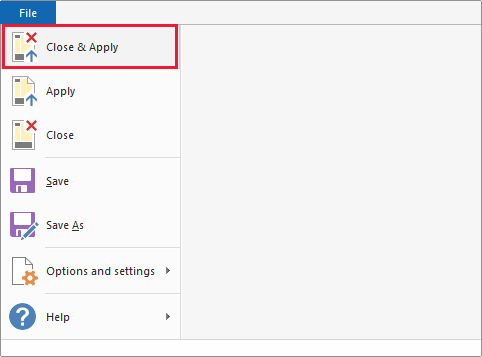
\includegraphics[width=\linewidth,height=4.2cm,keepaspectratio]{ms-learn/cerrar-y-aplicar.png}
    \fuente{Descripción general de consultas en Power BI Desktop}{\urlconsultas}
    \column{0.57\textwidth}
    \small
    \begin{enumerate}
      \small
      \item \menu{Archivo}{File} $>$ \menu{Cerrar y aplicar}{Close \&
        Apply}, o el mismo botón en la pestaña \menu{Inicio}{Home}.
      \item Power BI ejecuta los pasos y carga las cinco tablas en el
        modelo.
      \item Guarda: \menu{Archivo}{File} $>$ \menu{Guardar}{Save}, con
        el nombre \texttt{gimnasio\_vitalis}. Power BI le agrega la
        extensión \texttt{.pbix}.
      \item En la vista \textbf{Tabla}, revisa que \texttt{Socios} tenga
        \textbf{300 filas}.
    \end{enumerate}
    \begin{alertblock}{Cerrar y aplicar no es definitivo}
      \footnotesize Puedes volver a Power Query cuando quieras, corregir
      un paso y aplicar de nuevo.
    \end{alertblock}
  \end{columns}
\end{frame}

% ============================================================
\section{Hora 3: El modelo de datos}
% ============================================================
\begin{frame}[t]{Hechos y dimensiones}
  \begin{columns}[T,onlytextwidth]
    \column{0.48\textwidth}
    \begin{block}{Tabla de dimensión}
      \small Describe las cosas del negocio: \textbf{quién, qué, dónde,
      cuándo}. Pocas filas, una por cosa, con una llave única.\\[2pt]
      \footnotesize Ejemplos: \texttt{Socios}, \texttt{Planes},
      \texttt{Sedes}, \texttt{Calendario}.
    \end{block}
    \column{0.48\textwidth}
    \begin{alertblock}{Tabla de hechos}
      \small Registra \textbf{eventos}: cada pago, cada entrada. Muchas
      filas, que crecen con el tiempo, con números para sumar y llaves
      hacia las dimensiones.\\[2pt]
      \footnotesize Ejemplos: \texttt{Pagos}, \texttt{Asistencias}.
    \end{alertblock}
  \end{columns}
  \vspace{0.2cm}
  \small La pregunta que decide el tipo de una tabla: \textbf{¿qué es una
  fila?} Si es un evento que ocurrió en un momento, es de hechos. Si es una
  cosa que existe, de dimensión.
  \vspace{0.1cm}

  \footnotesize Los objetos visuales \textbf{agrupan} por columnas de
  dimensión (sede, plan, sexo) y \textbf{suman} columnas de hechos
  (valor pagado): es el \texttt{groupby} de la Clase 9.
\end{frame}

\begin{frame}[t]{El modelo estrella del Gimnasio Vitalis}
  \begin{center}
  \begin{tikzpicture}[
    tabla/.style={rectangle split, rectangle split parts=2, draw=esumerNavy, line width=0.6pt,
                  rounded corners=2pt, text width=2.45cm, align=left, font=\tiny\ttfamily,
                  inner sep=2.5pt, rectangle split part align={center,left}},
    dim/.style={tabla, rectangle split part fill={esumerTeal,white}},
    hec/.style={tabla, rectangle split part fill={esumerOrange,white}},
    rel/.style={line width=0.8pt, color=esumerNavy},
    card/.style={font=\scriptsize\bfseries, text=esumerNavy, fill=esumerBg, inner sep=1pt},
  ]
    \node[hec] (pagos) at (3.9,0) {\textcolor{white}{\bfseries\scriptsize\sffamily Pagos}\nodepart{two}id\_pago\\fecha\_pago\\id\_socio\\id\_plan\\id\_sede\\valor\_pagado\_cop\\medio\_pago};
    \node[hec] (asis) at (10.5,0) {\textcolor{white}{\bfseries\scriptsize\sffamily Asistencias}\nodepart{two}id\_asistencia\\id\_socio\\id\_sede\\fecha\\hora\_entrada\\duracion\_min};
    \node[dim] (socios) at (7.2,2.05) {\textcolor{white}{\bfseries\scriptsize\sffamily Socios}\nodepart{two}id\_socio\\nombre, sexo, edad\\grupo\_edad, activo\ldots};
    \node[dim] (sedes) at (7.2,0) {\textcolor{white}{\bfseries\scriptsize\sffamily Sedes}\nodepart{two}id\_sede\\sede, ciudad};
    \node[dim] (cal) at (7.2,-2.0) {\textcolor{white}{\bfseries\scriptsize\sffamily Calendario}\nodepart{two}Date\\Año, Mes, Año-Mes};
    \node[dim] (planes) at (0.75,0) {\textcolor{white}{\bfseries\scriptsize\sffamily Planes}\nodepart{two}id\_plan\\plan, meses\\precio\_lista\_cop};
    \foreach \d/\h in {socios/pagos, sedes/pagos, cal/pagos, planes/pagos, socios/asis, sedes/asis, cal/asis} {
      \draw[rel] (\d) -- (\h) node[card, pos=0.14] {1} node[card, pos=0.86] {*};
    }
  \end{tikzpicture}
  \end{center}
  \vspace{-0.15cm}
  \footnotesize Naranja: tablas de hechos. Verde: dimensiones. Cada línea
  une la llave de una dimensión (lado \textbf{1}) con la columna del mismo
  nombre en los hechos (lado \textbf{*}). \texttt{Calendario} la creas tú en
  el paso 16.
\end{frame}

\begin{frame}[t]{\npaso{14}\; Abrir la vista Modelo}
  \begin{columns}[T,onlytextwidth]
    \column{0.15\textwidth}
    \centering
    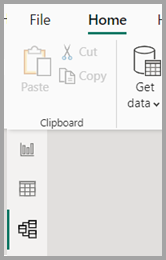
\includegraphics[width=\linewidth,height=3.2cm,keepaspectratio]{ms-learn/icono-vista-modelo.png}
    \column{0.42\textwidth}
    \centering
    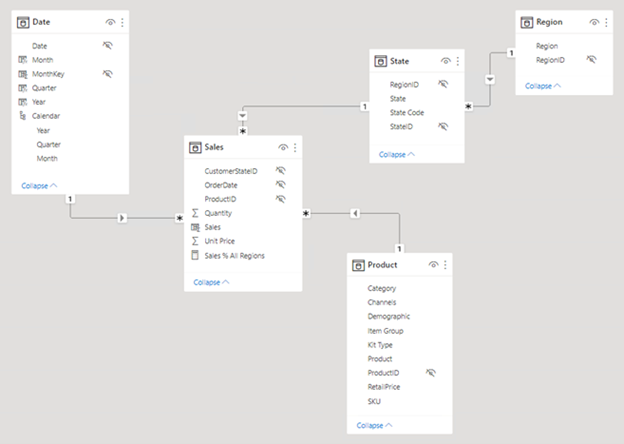
\includegraphics[width=\linewidth,height=3.6cm,keepaspectratio]{ms-learn/diagrama-modelo-estrella.png}
    \par\vspace{1pt}{\fontsize{5.5}{6.5}\selectfont\color{black!55}Capturas de Microsoft Power BI Desktop. Fuente: Microsoft Learn, \href{https://learn.microsoft.com/es-es/power-bi/transform-model/desktop-modeling-view}{«Uso de la vista Modelo»} y \href{\urlrelentender}{«Relaciones de modelo»}. Used with permission from Microsoft.\par}
    \column{0.4\textwidth}
    \small
    \begin{enumerate}
      \small
      \item Haz clic en el tercer ícono de la izquierda, el de tablas
        conectadas: vista \textbf{Modelo}.
      \item Arrastra cada tabla por su título hasta formar la estrella,
        con los hechos al centro.
      \item Power BI ya creó \textbf{algunas relaciones solo}, uniendo
        columnas con el mismo nombre. Haz clic en cada línea para ver qué
        columnas une.
    \end{enumerate}
  \end{columns}
  \vspace{0.1cm}
  \footnotesize Al centro, el modelo de ejemplo de Microsoft: la misma
  forma de estrella que el nuestro.
\end{frame}

\begin{frame}[t]{\npaso{15}\; Crear o corregir una relación}
  \begin{columns}[T,onlytextwidth]
    \column{0.48\textwidth}
    \centering
    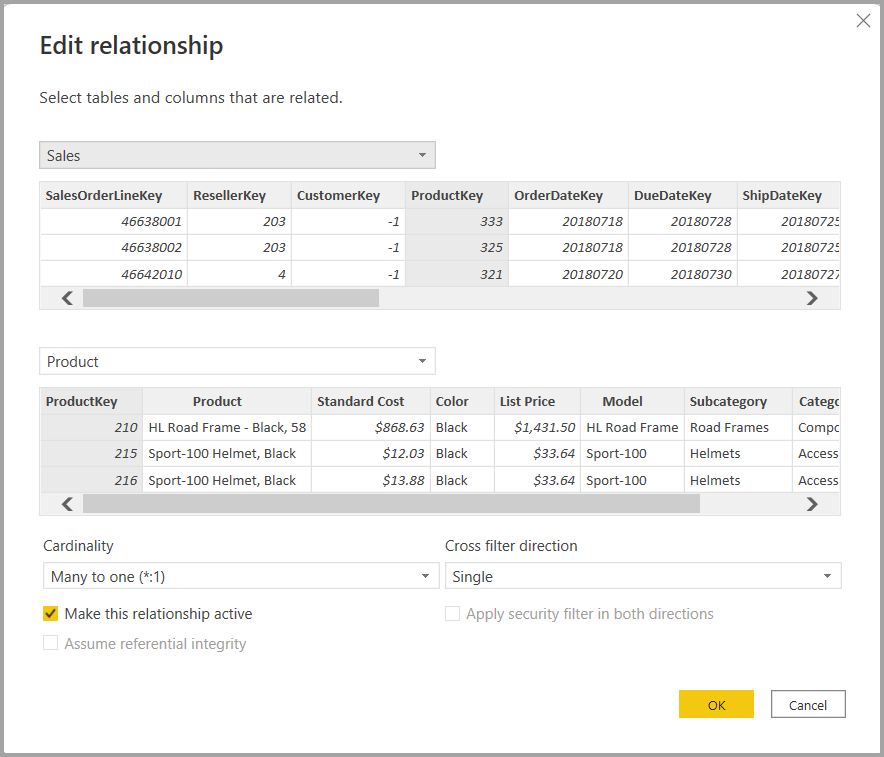
\includegraphics[width=\linewidth,height=4.6cm,keepaspectratio]{ms-learn/ventana-editar-relacion.png}
    \fuente{Creación y administración de relaciones en Power BI Desktop}{https://learn.microsoft.com/es-es/power-bi/transform-model/desktop-create-and-manage-relationships}
    \column{0.49\textwidth}
    \small
    \footnotesize Dos formas de crearla:
    \begin{itemize}
      \footnotesize
      \item En la vista Modelo, \textbf{arrastra} \texttt{id\_socio} de
        \texttt{Pagos} hasta \texttt{id\_socio} de \texttt{Socios}.
      \item O en la cinta, \menu{Administrar relaciones}{Manage
        relationships} $>$ \menu{Nueva}{New}.
    \end{itemize}
    En la ventana, comprueba:
    \begin{enumerate}
      \footnotesize
      \item Las dos tablas y las dos columnas correctas.
      \item Cardinalidad: \menu{Varios a uno}{Many to one (*:1)}, o Uno
        a varios (1:*) si pusiste primero \texttt{Socios}: es lo mismo.
      \item Filtro cruzado: \menu{Único}{Single}.
      \item Activa: marcada.
    \end{enumerate}
  \end{columns}
\end{frame}

\begin{frame}[t]{Cardinalidad: qué significan el 1 y el *}
  \begin{columns}[T,onlytextwidth]
    \column{0.5\textwidth}
    \centering
    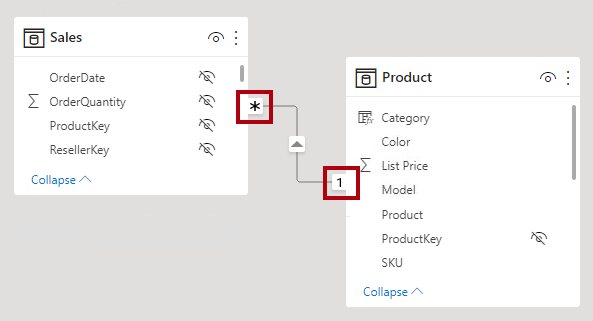
\includegraphics[width=\linewidth,height=4.0cm,keepaspectratio]{ms-learn/cardinalidad.png}
    \fuente{Relaciones de modelo en Power BI Desktop}{\urlrelentender}
    \column{0.47\textwidth}
    \small
    Los símbolos en los extremos de la línea dicen cuántas filas pueden
    emparejarse:
    \begin{itemize}
      \small
      \item \textbf{1}: la llave es única en esa tabla. Un socio aparece
        una sola vez en \texttt{Socios}.
      \item \textbf{*} (varios): la columna puede repetirse. Un socio tiene
        muchos pagos.
    \end{itemize}
    \begin{exampleblock}{En pandas (Clase 10)}
      \footnotesize Es el \texttt{validate="many\_to\_one"} del
      \texttt{merge}: Power BI comprueba la misma condición al crear la
      relación.
    \end{exampleblock}
  \end{columns}
\end{frame}

\begin{frame}[t]{Dirección del filtro cruzado}
  \begin{columns}[T,onlytextwidth]
    \column{0.5\textwidth}
    \centering
    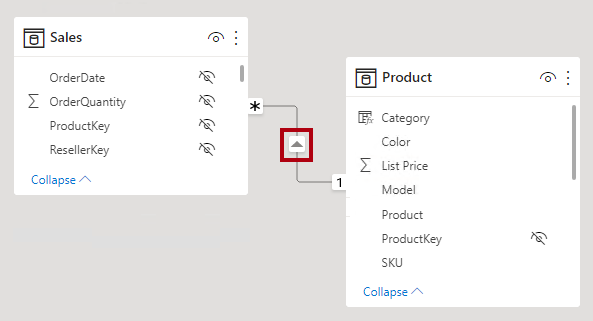
\includegraphics[width=\linewidth,height=4.0cm,keepaspectratio]{ms-learn/direccion-filtro.png}
    \fuente{Relaciones de modelo en Power BI Desktop}{\urlrelentender}
    \column{0.47\textwidth}
    \small
    La flecha sobre la línea indica hacia dónde viaja un filtro.
    \begin{itemize}
      \small
      \item \textbf{Único}: el filtro va de la dimensión (1) a los hechos
        (*). Si eliges la sede Poblado, solo se suman los pagos de esa
        sede.
      \item \textbf{Ambos}: el filtro viaja en las dos direcciones.
    \end{itemize}
    \begin{alertblock}{Deja Único}
      \footnotesize En un modelo estrella, Único es casi siempre lo
      correcto. Ambos puede crear caminos ambiguos y resultados difíciles
      de explicar.
    \end{alertblock}
  \end{columns}
\end{frame}

\begin{frame}[t]{Las relaciones de nuestro modelo}
  \small
  Al terminar la Hora 3 debes tener exactamente estas siete relaciones,
  todas varios a uno, de filtro único y activas:
  \vspace{0.15cm}

  \footnotesize
  \renewcommand{\arraystretch}{1.1}
  \begin{columns}[T,onlytextwidth]
    \column{0.55\textwidth}
    \begin{tabular}{@{}ll@{}}
      \toprule
      \textbf{Hechos (lado *)} & \textbf{Dimensión (lado 1)} \\
      \midrule
      \texttt{Pagos[id\_socio]} & \texttt{Socios[id\_socio]} \\
      \texttt{Pagos[id\_plan]} & \texttt{Planes[id\_plan]} \\
      \texttt{Pagos[id\_sede]} & \texttt{Sedes[id\_sede]} \\
      \texttt{Pagos[fecha\_pago]} & \texttt{Calendario[Date]} \\
      \texttt{Asistencias[id\_socio]} & \texttt{Socios[id\_socio]} \\
      \texttt{Asistencias[id\_sede]} & \texttt{Sedes[id\_sede]} \\
      \texttt{Asistencias[fecha]} & \texttt{Calendario[Date]} \\
      \bottomrule
    \end{tabular}
    \column{0.42\textwidth}
    \small
    Ninguna relación une dos dimensiones entre sí, ni dos tablas de
    hechos entre sí.
    \vspace{0.15cm}

    \small Las dos de \texttt{Calendario} las creas en el paso 16.
    \vspace{0.15cm}

    \small Si ves una línea \textbf{punteada}, es una relación inactiva:
    Power BI la desactivó porque encontró dos caminos posibles entre las
    mismas tablas. Revisa cuál sobra y elimínala.
  \end{columns}
\end{frame}

\begin{frame}[t]{Si la relación no se deja crear}
  \small
  Casi siempre es por algo que ya viste en el Módulo 2:
  \vspace{0.15cm}

  \footnotesize
  \renewcommand{\arraystretch}{1.2}
  \begin{tabular}{@{}L{4.0cm}L{4.9cm}L{3.9cm}@{}}
    \toprule
    \textbf{Lo que ves} & \textbf{La causa} & \textbf{La solución} \\
    \midrule
    Power BI solo ofrece varios a varios (*:*) & la llave de la dimensión tiene duplicados & paso 5, en Power Query \\
    Error de tipos al crear la relación & una columna es texto y la otra número & paso 6, en las dos tablas \\
    La relación existe, pero los totales no cambian por sede o plan & valores que no coinciden (\texttt{"Itagui"} frente a \texttt{"Itagüí"}) & normalizar la llave, como en la Clase 10 \\
    Una relación aparece punteada & dos caminos posibles entre dos tablas & eliminar la relación que sobra \\
    \bottomrule
  \end{tabular}
\end{frame}

\begin{frame}[t]{\npaso{16}\; Una tabla de fechas: \texttt{Calendario} (1/2)}
  \begin{columns}[T,onlytextwidth]
    \column{0.42\textwidth}
    \centering
    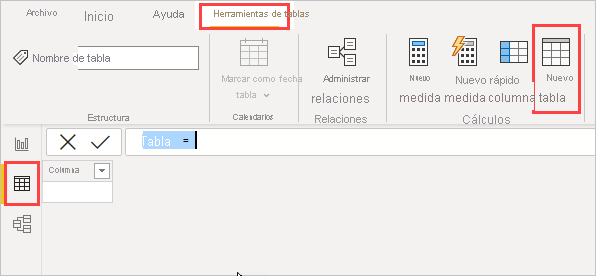
\includegraphics[width=\linewidth,height=2.7cm,keepaspectratio]{ms-learn/nueva-tabla.png}
    \fuente{Uso de tablas calculadas en Power BI Desktop}{https://learn.microsoft.com/es-es/power-bi/transform-model/desktop-calculated-tables}
    \vspace{0.1cm}
    \raggedright\footnotesize\textbf{¿Para qué?} Pagos y Asistencias
    tienen sus propias fechas. Con una sola tabla de fechas unida a las
    dos, un mismo filtro (por ejemplo, marzo de 2026) recorta ambas.
    \column{0.55\textwidth}
    \footnotesize
    \begin{enumerate}
      \footnotesize
      \item Vista \textbf{Tabla}: \menu{Herramientas de tabla}{Table
        tools} $>$ \menu{Nueva tabla}{New table}.
      \item Arriba aparece la barra de fórmulas con \texttt{Tabla =}.
        Borra ese texto, escribe esto y presiona Enter:
    \end{enumerate}
    \vspace{-0.15cm}
    \codigo{Calendario = CALENDAR(\\
      \hspace*{1em}DATE(2025, 9, 1), DATE(2026, 9, 30))}
    \begin{enumerate}
      \footnotesize
      \setcounter{enumi}{2}
      \item Resultado: una tabla con una sola columna, \texttt{Date}, y
        una fila por cada día entre esas dos fechas.
      \item Clic derecho en \texttt{Calendario} (panel Datos) $>$
        \menu{Marcar como tabla de fechas}{Mark as date table}, y elige la
        columna \texttt{Date}.
      \item En la vista Modelo, arrastra \texttt{Date} hasta
        \texttt{Pagos[fecha\_pago]} y luego hasta
        \texttt{Asistencias[fecha]}.
    \end{enumerate}
  \end{columns}
\end{frame}

\begin{frame}[t]{\npaso{16}\; Una tabla de fechas: \texttt{Calendario} (2/2)}
  \small
  Para agrupar por año o por mes en los gráficos de la Clase 14, agrega
  tres columnas a \texttt{Calendario}. Con la tabla seleccionada:
  \menu{Herramientas de tabla}{Table tools} $>$ \menu{Nueva
  columna}{New column}, una vez por cada fórmula (escríbela y presiona
  Enter):
  \vspace{0.1cm}
  \codigo{Año = YEAR(Calendario[Date])\\[2pt]
    Mes = MONTH(Calendario[Date])\\[2pt]
    Año-Mes = FORMAT(Calendario[Date], "yyyy-mm")}
  \vspace{0.1cm}
  \begin{columns}[T,onlytextwidth]
    \column{0.45\textwidth}
    \footnotesize
    \begin{tabular}{@{}llll@{}}
      \toprule
      \textbf{Date} & \textbf{Año} & \textbf{Mes} & \textbf{Año-Mes} \\
      \midrule
      2025-09-01 & 2025 & 9 & 2025-09 \\
      2026-03-15 & 2026 & 3 & 2026-03 \\
      \bottomrule
    \end{tabular}
    \column{0.52\textwidth}
    \footnotesize Así se ven dos filas. \texttt{Año-Mes} sirve como eje de
    un gráfico de líneas por mes, como \texttt{dt.to\_period("M")} en la
    Clase 9.
  \end{columns}
\end{frame}

\begin{frame}[t]{Tres formas de calcular, y cuándo usar cada una}
  \footnotesize
  \renewcommand{\arraystretch}{1.25}
  \begin{tabular}{@{}L{1.9cm}L{3.3cm}L{3.5cm}L{4.0cm}@{}}
    \toprule
    & \textbf{Columna personalizada} & \textbf{Columna calculada} & \textbf{Medida} \\
    \midrule
    Dónde & Power Query & Modelo & Modelo \\
    Lenguaje & M & DAX & DAX \\
    Se calcula & al cargar o actualizar & al cargar, fila por fila & cada vez que un visual la usa, según los filtros \\
    Resultado & una columna más & una columna más & un solo número \\
    Ejemplo de hoy & \texttt{edad} (paso 10) & \texttt{descuento\_cop} (paso 17) & \texttt{Ingresos} (paso 18) \\
    Úsala para & limpiar y preparar datos & datos fila por fila que necesitan otra tabla del modelo & totales, promedios e indicadores clave (KPI) \\
    \bottomrule
  \end{tabular}

  \vspace{0.25cm}
  \small Regla práctica: \textbf{si es para sumar, contar o promediar, es
  una medida}. Las medidas son el \texttt{groupby().agg()} de Power BI: el
  objeto visual decide los grupos y la medida decide el cálculo.
\end{frame}

\begin{frame}[t]{\npaso{17}\; Columna calculada con DAX}
  \begin{columns}[T,onlytextwidth]
    \column{0.18\textwidth}
    \centering
    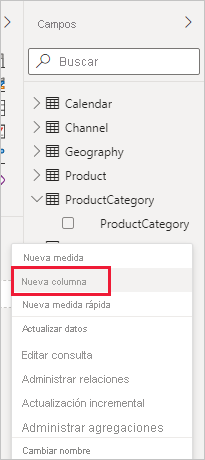
\includegraphics[width=\linewidth,height=4.1cm,keepaspectratio]{ms-learn/menu-nueva-columna.png}
    \column{0.42\textwidth}
    \centering
    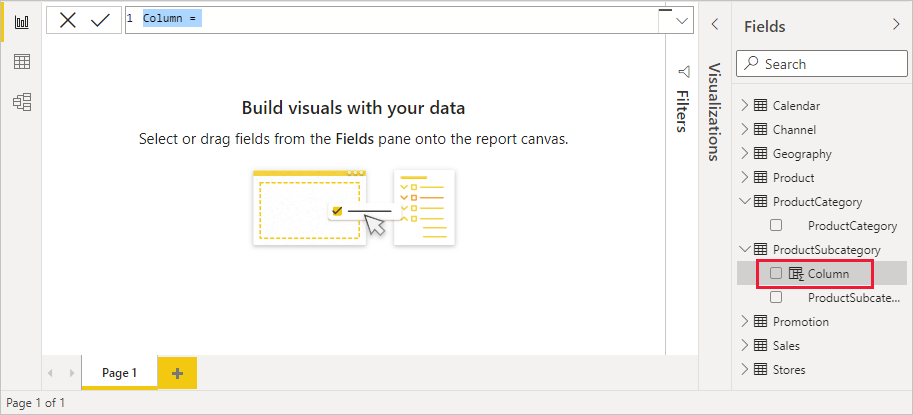
\includegraphics[width=\linewidth,height=2.8cm,keepaspectratio]{ms-learn/barra-formulas.png}
    \fuente{Tutorial: Creación de columnas calculadas en Power BI Desktop}{https://learn.microsoft.com/es-es/power-bi/transform-model/desktop-tutorial-create-calculated-columns}
    \column{0.37\textwidth}
    \small
    \begin{enumerate}
      \small
      \item En la vista Tabla, en el panel \textbf{Datos} (derecha), clic
        derecho en \texttt{Pagos} $>$ \menu{Nueva columna}{New column}.
      \item En la barra de fórmulas, borra \texttt{Columna =}, escribe
        esto y presiona Enter:
    \end{enumerate}
  \end{columns}
  \vspace{0.05cm}
  \codigo{descuento\_cop = RELATED(Planes[precio\_lista\_cop]) - Pagos[valor\_pagado\_cop]}
  \footnotesize \texttt{RELATED} trae, para cada pago, el precio de lista de
  su plan. Solo funciona si ya existe la relación entre \texttt{Pagos} y
  \texttt{Planes}: es un \texttt{merge} hecho por el modelo. Los pagos con la
  promoción de bienvenida muestran un descuento del 10\%.
\end{frame}

\begin{frame}[t]{\npaso{18}\; Tus primeras medidas}
  \begin{columns}[T,onlytextwidth]
    \column{0.37\textwidth}
    \centering
    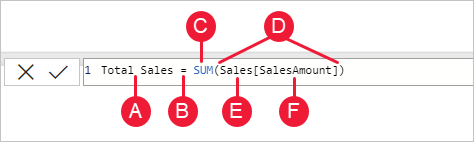
\includegraphics[width=\linewidth]{ms-learn/sintaxis-dax.png}
    \fuente{Aspectos básicos de DAX en Power BI Desktop}{https://learn.microsoft.com/es-es/power-bi/transform-model/desktop-quickstart-learn-dax-basics}
    \vspace{0.05cm}
    \raggedright\scriptsize A: nombre de la medida. B: signo igual. C:
    función. D: paréntesis con los argumentos. E: tabla. F: columna.
    \column{0.6\textwidth}
    \small
    En el panel Datos, clic derecho en \texttt{Pagos} $>$ \menu{Nueva
    medida}{New measure}; escribe la fórmula y presiona Enter. Repite para
    cada una (\texttt{Visitas}, en \texttt{Asistencias}):
    \vspace{0.05cm}
    \codigo{%
      Ingresos = SUM(Pagos[valor\_pagado\_cop])\\[2pt]
      Pagos realizados = COUNTROWS(Pagos)\\[2pt]
      Socios que pagaron = DISTINCTCOUNT(Pagos[id\_socio])\\[2pt]
      Pago promedio = DIVIDE([Ingresos], [Pagos realizados])\\[2pt]
      Visitas = COUNTROWS(Asistencias)}
    \footnotesize Las medidas aparecen en el panel Datos con un ícono de
    calculadora. \texttt{DIVIDE} evita el error de dividir entre cero.
  \end{columns}
\end{frame}

\begin{frame}[t]{\npaso{19}\; Comprueba el modelo con una tabla}
  \begin{columns}[T,onlytextwidth]
    \column{0.47\textwidth}
    \small
    \begin{enumerate}
      \scriptsize
      \item Vista \textbf{Informe} (primer ícono de la izquierda).
      \item En el panel Visualizaciones, clic en el ícono \textbf{Tabla}
        (una cuadrícula).
      \item En el panel Datos, marca \texttt{sede} (en \texttt{Sedes}) y
        \texttt{Ingresos} (en \texttt{Pagos}).
    \end{enumerate}
    \scriptsize Debes ver (quizá sin puntos de miles):
    \vspace{0.1cm}

    \scriptsize
    \renewcommand{\arraystretch}{0.95}
    \begin{tabular}{@{}lr@{}}
      \toprule
      \textbf{Sede} & \textbf{Ingresos (COP)} \\
      \midrule
      Sede Poblado & 70.847.000 \\
      Sede Chapinero & 52.458.000 \\
      Sede Envigado & 43.991.000 \\
      Sede Itagüí & 15.021.000 \\
      Sede Cali & 10.107.000 \\
      \midrule
      \textbf{Total} & \textbf{192.424.000} \\
      \bottomrule
    \end{tabular}
    \column{0.5\textwidth}
    \begin{alertblock}{Si todas las sedes muestran 192.424.000}
      \footnotesize Falta la relación entre \texttt{Pagos} y
      \texttt{Sedes}, o está inactiva: el filtro de la sede no llega a los
      pagos y cada fila muestra el total.
    \end{alertblock}
    \small Otras cifras para comprobar:
    \begin{itemize}
      \footnotesize
      \item 1396 pagos realizados y 300 socios que pagaron.
      \item 17083 visitas.
      \item Ingresos por plan: Mensual 105.426.000, Trimestral 35.328.000,
        Anual 43.120.000, Semestral 8.550.000.
    \end{itemize}
  \end{columns}
\end{frame}

\begin{frame}[t]{Checklist: el modelo está listo cuando\ldots}
  \small
  \begin{enumerate}
    \item \texttt{Socios} tiene 300 filas, sin duplicados, y \texttt{sexo}
      solo tiene tres valores.
    \item Las columnas tienen el tipo correcto: llaves como número entero,
      teléfono como texto, fechas como fecha.
    \item Hay seis tablas: cuatro dimensiones y dos de hechos.
    \item Las siete relaciones son varios a uno, de filtro único, y
      ninguna está punteada.
    \item \texttt{Calendario} está marcada como tabla de fechas.
    \item Las cinco medidas existen y la tabla del paso 19 coincide con
      las cifras de control.
    \item Los pasos de Power Query tienen nombres que explican qué hacen.
  \end{enumerate}
\end{frame}

% ============================================================
\section{Taller}
% ============================================================
\begin{frame}[t]{Actividad práctica}
  \begin{columns}[T,onlytextwidth]
    \column{0.48\textwidth}
    \begin{block}{Parte A: el gimnasio (en clase)}
      \small Sigue los pasos 1 a 19 de esta guía con
      \texttt{gimnasio\_vitalis.xlsx}, hasta que la tabla del paso 19
      coincida con las cifras de control.
    \end{block}
    \column{0.48\textwidth}
    \begin{alertblock}{Parte B: tu proyecto}
      \small Repite el proceso con tus datos (puedes partir del CSV limpio
      que guardaste en la Clase 12):
      \begin{enumerate}
        \footnotesize
        \item Clasifica cada tabla como hechos o dimensión, y di qué es
          una fila.
        \item Haz al menos tres pasos de limpieza en Power Query.
        \item Crea las relaciones y una tabla de fechas.
        \item Crea tres medidas y una tabla que las compruebe.
      \end{enumerate}
    \end{alertblock}
  \end{columns}
  \vspace{0.05cm}
  \footnotesize ¿Tu proyecto tiene una sola tabla? Las columnas que se
  repiten en muchas filas (cliente, producto, sede) son candidatas a
  dimensión.
\end{frame}

\begin{frame}[t]{Producto esperado}
  \begin{exampleblock}{Entregable}
    \small
    \begin{enumerate}
      \item El archivo \texttt{.pbix} con el modelo de tu proyecto.
      \item Una captura de la vista Modelo, con las relaciones visibles
        (en Windows: tecla Windows + Mayús + S).
      \item La bitácora de decisiones de la Clase 12, ampliada con los
        pasos de Power Query: qué encontraste, qué paso aplicaste y por
        qué.
    \end{enumerate}
  \end{exampleblock}
  \small Este archivo es el punto de partida de la Clase 14: ahí vas a
  construir el tablero encima de este modelo.
\end{frame}

% ============================================================
\section{Cierre}
% ============================================================
\begin{frame}[t]{Cierre y próxima sesión}
  \begin{itemize}
    \item Power Query es el pipeline de limpieza del Módulo 2 hecho con
      clics: cada clic es un paso guardado, y el archivo original nunca
      cambia.
    \item Un buen modelo separa las tablas que describen (dimensiones) de
      las que registran eventos (hechos), y las une con relaciones varios a
      uno.
    \item Las medidas son el \texttt{groupby} de Power BI: se calculan
      según lo que filtre cada objeto visual.
    \item Próxima sesión, \textbf{Clase 14: Dashboard e identificación de
      insights}: gráficos de barras, líneas, dispersión y mapas sobre este
      modelo.
  \end{itemize}
\end{frame}

\begin{frame}[t]{Documentación oficial usada en cada paso}
  \scriptsize
  Todas las páginas son de Microsoft Learn, en español. Haz clic en el
  título para abrirla.
  \vspace{0.1cm}
  \renewcommand{\arraystretch}{1.08}
  \begin{columns}[T,onlytextwidth]
    \column{0.49\textwidth}
    \begin{tabular}{@{}L{1.4cm}L{4.95cm}@{}}
      \toprule
      \textbf{Paso} & \textbf{Página oficial} \\
      \midrule
      Instalar & \href{\urlinstalar}{\color{esumerOrange}Descarga de Power BI Desktop} \\
      1 a 3 & \href{\urlconectar}{\color{esumerOrange}Inicio rápido: conexión a datos} \\
      Hora 2 & \href{\urlconsultas}{\color{esumerOrange}Descripción general de consultas (Power Query)} \\
      4 & \href{https://learn.microsoft.com/es-es/power-query/data-profiling-tools}{\color{esumerOrange}Herramientas de generación de perfiles de datos} \\
      5 & \href{https://learn.microsoft.com/es-es/power-query/working-with-duplicates}{\color{esumerOrange}Trabajar con valores duplicados} \\
      6 & \href{https://learn.microsoft.com/es-es/power-query/data-types}{\color{esumerOrange}Tipos de datos en Power Query} \\
      7 a 9 & \href{https://learn.microsoft.com/es-es/power-query/replace-values}{\color{esumerOrange}Reemplazar valores y errores} \\
      10 & \href{https://learn.microsoft.com/es-es/power-query/add-custom-column}{\color{esumerOrange}Adición de una columna personalizada} \\
      11 & \href{https://learn.microsoft.com/es-es/power-query/add-conditional-column}{\color{esumerOrange}Agregar columna condicional} \\
      12 & \href{https://learn.microsoft.com/es-es/power-query/merge-queries-overview}{\color{esumerOrange}Consultas de combinación} y \href{https://learn.microsoft.com/es-es/power-query/merge-queries-left-outer}{\color{esumerOrange}combinación externa izquierda} \\
      \bottomrule
    \end{tabular}
    \column{0.49\textwidth}
    \begin{tabular}{@{}L{1.4cm}L{4.95cm}@{}}
      \toprule
      \textbf{Paso} & \textbf{Página oficial} \\
      \midrule
      Hora 3 & \href{https://learn.microsoft.com/es-es/power-bi/guidance/star-schema}{\color{esumerOrange}Comprender el esquema de estrella} \\
      14 & \href{https://learn.microsoft.com/es-es/power-bi/transform-model/desktop-modeling-view}{\color{esumerOrange}Uso de la vista Modelo} \\
      15 & \href{https://learn.microsoft.com/es-es/power-bi/transform-model/desktop-create-and-manage-relationships}{\color{esumerOrange}Creación y administración de relaciones} \\
      15 & \href{\urlrelentender}{\color{esumerOrange}Relaciones de modelo (cardinalidad y filtro cruzado)} \\
      16 & \href{https://learn.microsoft.com/es-es/power-bi/transform-model/desktop-calculated-tables}{\color{esumerOrange}Tablas calculadas}, \href{https://learn.microsoft.com/es-es/dax/calendar-function-dax}{\color{esumerOrange}función CALENDAR} y \href{https://learn.microsoft.com/es-es/power-bi/transform-model/desktop-date-tables}{\color{esumerOrange}tablas de fechas} \\
      17 & \href{https://learn.microsoft.com/es-es/power-bi/transform-model/desktop-tutorial-create-calculated-columns}{\color{esumerOrange}Tutorial: columnas calculadas} \\
      18 & \href{https://learn.microsoft.com/es-es/power-bi/transform-model/desktop-quickstart-learn-dax-basics}{\color{esumerOrange}Aspectos básicos de DAX} y \href{https://learn.microsoft.com/es-es/power-bi/transform-model/desktop-measures}{\color{esumerOrange}medidas} \\
      Vistas & \href{https://learn.microsoft.com/es-es/power-bi/transform-model/dax-query-view}{\color{esumerOrange}Vista de consultas DAX (el cuarto ícono)} \\
      \bottomrule
    \end{tabular}
  \end{columns}
\end{frame}

\begin{frame}[t]{Para seguir aprendiendo}
  \footnotesize
  \begin{columns}[T,onlytextwidth]
    \column{0.52\textwidth}
    \textbf{Módulos de Microsoft Learn, en español}
    \begin{itemize}
      \footnotesize
      \item \href{https://learn.microsoft.com/es-es/training/modules/get-data/}{\color{esumerOrange}Obtener datos en Power BI}
      \item \href{https://learn.microsoft.com/es-es/training/modules/clean-data-power-bi/}{\color{esumerOrange}Limpiar, transformar y cargar datos en Power BI}
      \item \href{https://learn.microsoft.com/es-es/training/modules/design-model-power-bi/}{\color{esumerOrange}Configurar un modelo semántico en Power BI Desktop}
      \item \href{https://learn.microsoft.com/es-es/training/modules/dax-power-bi-write-formulas/}{\color{esumerOrange}Escribir fórmulas DAX para modelos semánticos}
    \end{itemize}
    \textbf{Documentación oficial, en español}
    \begin{itemize}
      \footnotesize
      \item \href{\urlconsultas}{\color{esumerOrange}Descripción general de consultas (Power Query)}
      \item \href{https://learn.microsoft.com/es-es/power-bi/guidance/star-schema}{\color{esumerOrange}Comprender el esquema de estrella}
      \item \href{https://learn.microsoft.com/es-es/dax/}{\color{esumerOrange}Referencia de funciones DAX}
    \end{itemize}
    \column{0.45\textwidth}
    \textbf{Descargas}
    \begin{itemize}
      \footnotesize
      \item \href{https://apps.microsoft.com/detail/9ntxr16hnw1t?hl=es-co}{\color{esumerOrange}Power BI Desktop en Microsoft Store}
      \item \href{https://www.microsoft.com/download/details.aspx?id=58494}{\color{esumerOrange}Power BI Desktop en el Centro de descargas}
      \item \href{\urldatos}{\color{esumerOrange}Datos de la clase: gimnasio\_vitalis.xlsx}
    \end{itemize}
    \textbf{Otras guías (en inglés)}
    \begin{itemize}
      \footnotesize
      \item SQLBI, \href{https://www.sqlbi.com/p/introducing-dax-video-course/}{\color{esumerOrange}Introducing DAX}:
        curso gratuito en video de los autores de referencia en DAX.
      \item SQLBI, \href{https://www.sqlbi.com/articles/power-bi-star-schema-or-single-table/}{\color{esumerOrange}Star schema or single table}:
        por qué separar en hechos y dimensiones.
      \item SQLBI, \href{https://www.sqlbi.com/articles/understanding-relationships-in-power-bi/}{\color{esumerOrange}Understanding relationships in Power BI}.
    \end{itemize}
  \end{columns}
\end{frame}

\begin{frame}[t]{Créditos de las imágenes}
  \scriptsize
  Las capturas de pantalla de Microsoft Power BI Desktop provienen de la
  documentación de Microsoft Learn y se reproducen sin modificaciones,
  conforme a la política de Microsoft sobre capturas de pantalla de sus
  productos. \textbf{Used with permission from Microsoft.}
  \vspace{0.15cm}

  Páginas de origen:
  \begin{itemize}
    \scriptsize
    \item \href{https://learn.microsoft.com/es-es/power-bi/fundamentals/desktop-get-the-desktop}{Descarga de Power BI Desktop}
      \textperiodcentered\ \href{\urlconectar}{Inicio rápido: Conexión a datos}
      \textperiodcentered\ \href{\urlconsultas}{Descripción general de consultas}
    \item \href{https://learn.microsoft.com/es-es/power-query/data-profiling-tools}{Herramientas de generación de perfiles de datos}
      \textperiodcentered\ \href{https://learn.microsoft.com/es-es/power-query/working-with-duplicates}{Trabajar con valores duplicados}
      \textperiodcentered\ \href{https://learn.microsoft.com/es-es/power-query/data-types}{Tipos de datos en Power Query}
    \item \href{https://learn.microsoft.com/es-es/power-query/replace-values}{Reemplazar valores y errores}
      \textperiodcentered\ \href{https://learn.microsoft.com/es-es/power-query/add-custom-column}{Columna personalizada}
      \textperiodcentered\ \href{https://learn.microsoft.com/es-es/power-query/add-conditional-column}{Columna condicional}
      \textperiodcentered\ \href{https://learn.microsoft.com/es-es/power-query/merge-queries-overview}{Consultas de combinación}
    \item \href{https://learn.microsoft.com/es-es/power-bi/transform-model/desktop-modeling-view}{Vista Modelo}
      \textperiodcentered\ \href{\urlrelentender}{Relaciones de modelo}
      \textperiodcentered\ \href{https://learn.microsoft.com/es-es/power-bi/transform-model/desktop-create-and-manage-relationships}{Creación y administración de relaciones}
    \item \href{https://learn.microsoft.com/es-es/power-bi/transform-model/desktop-calculated-tables}{Tablas calculadas}
      \textperiodcentered\ \href{https://learn.microsoft.com/es-es/power-bi/transform-model/desktop-tutorial-create-calculated-columns}{Columnas calculadas}
      \textperiodcentered\ \href{https://learn.microsoft.com/es-es/power-bi/transform-model/desktop-quickstart-learn-dax-basics}{Aspectos básicos de DAX}
  \end{itemize}
  \vspace{0.1cm}
  Los datos del Gimnasio Vitalis son ficticios, creados para el curso.
\end{frame}

{
\setbeamertemplate{footline}{}
\begin{frame}[plain,noframenumbering]
  \begin{tikzpicture}[remember picture,overlay]
    \fill[esumerNavy] (current page.south west) rectangle (current page.north east);
    \node at (current page.center) {\color{white}\Huge\bfseries ¡Gracias!};
  \end{tikzpicture}
\end{frame}
}

\end{document}
